\documentclass[acmsmall,screen,dvipsnames,x11names,nonacm,anonymous,review]{acmart}
\usepackage[most]{tcolorbox}
\usepackage{listings}
\usepackage{caption}
\usepackage{cleveref}
% Redefine sections to display with § symbol
\crefformat{section}{\S#2#1#3}
\Crefformat{section}{\S#2#1#3}

% Ensure subsections/subsubsections behave the same way (optional)
\crefformat{subsection}{\S#2#1#3}
\Crefformat{subsection}{\S#2#1#3}
\crefformat{subsubsection}{\S#2#1#3}
\Crefformat{subsubsection}{\S#2#1#3}

\usepackage[table,xcdraw]{xcolor}
\usepackage{tikz}
\usetikzlibrary{fit,positioning,calc}
\definecolor{col1}{HTML}{90f1ef}
\definecolor{col2}{HTML}{ffd6e0}
\definecolor{col3}{HTML}{ffef9f}

\definecolor{typecolor}{HTML}{4169E1} % RoyalBlue
\newcommand{\codetype}[1]{\textcolor{typecolor}{\ttfamily\small#1}}
% Macros for float type notation with proper braces
% Use \ftb{bounds}{values} for float type with both bounds and values
% Use \ft{bounds} for float type with bounds and T for values
% Use \ftt for float[T; T]
\newcommand{\ftb}[2]{\codetype{float[\{#1\}; \{#2\}]}}  % Both bags have values
\newcommand{\ft}[1]{\codetype{float[\{#1\}; T]}}        % Bounds only, values are T
\newcommand{\ftt}{\codetype{float[T; T]}}               % Both bags are T
\newcommand{\ftv}[1]{\codetype{float[T; \{#1\}]}}       % Bounds are T, values specified
% Macros for finite type operations and boolean operators
\newcommand{\finconst}[2]{#1_{\##2}}                    % k_{#n}
\newcommand{\finlt}[1]{<_{\#{#1}}}                      % <#n with subscript
\newcommand{\finleq}[1]{\leq_{\#{#1}}}                  % <=#n with subscript
\newcommand{\logand}{\mathrel{\&\&}}                    % logical and
\newcommand{\logor}{\mathrel{||}}                       % logical or

\renewcommand{\paragraph}[1]{\vspace{1em}\noindent\textbf{#1}\ }

\newcommand{\alexandra}[1]{\textcolor{pink}{\textbf{Alexandra:} #1}}
\newcommand{\kevin}[1]{\textcolor{ForestGreen}{\textbf{Kevin:} #1}}
\newcommand{\katherine}[1]{\textcolor{Purple}{\textbf{Katherine:} #1}}
\newcommand{\jules}[1]{\textcolor{blue}{\textbf{Jules:} #1}}




\tcbuselibrary{listingsutf8}

\newtcblisting{mybox}[2][]{%
  colback=#2!20,
  colframe=#2!80!black,
  coltitle=white,
  boxrule=1pt,
  arc=6pt,
  fonttitle=\bfseries\footnotesize,
  listing only,
  listing options={
    basicstyle=\ttfamily\footnotesize,
    breaklines=true,
    language=Dice,
    showstringspaces=false
  },
  width=\linewidth,
  valign=top,
  height=3.6cm,
  #1
}
\usepackage[scaled=0.84]{beramono}
\usepackage{mathpartir}
\usepackage{xspace}
\usepackage{todonotes}
\usepackage{subcaption}
\title{Slice: Type-Directed Discretization of Continuous Probabilistic Programs}

\lstdefinelanguage{Dice}{
    morekeywords={let, in, if, then, else, fst, snd, fun},
    morekeywords=[2]{uniform, discrete, gaussian, exponential, beta},
    morekeywords=[3]{bool, float, int},
    basicstyle=\ttfamily\small,
    keywordstyle=\bfseries,
    commentstyle=\itshape,
    stringstyle=\ttfamily,
    lineskip=-1pt,                
    aboveskip=0.1em,                
    belowskip=0.1em,
}




% Macros for language keywords to be used in math mode
\newcommand{\letkw}{\text{\ttfamily\bfseries let}}
\newcommand{\inkw}{\text{\ttfamily\bfseries in}}
\newcommand{\ifkw}{\text{\ttfamily\bfseries if}}
\newcommand{\thenkw}{\text{\ttfamily\bfseries then}}
\newcommand{\elsekw}{\text{\ttfamily\bfseries else}}
\newcommand{\uniform}{\text{\ttfamily\bfseries uniform}}
\newcommand{\discrete}{\text{\ttfamily\bfseries discrete}}
\newcommand{\gaussian}{\text{\ttfamily\bfseries gaussian}}
\newcommand{\exponential}{\text{\ttfamily\bfseries exponential}}
\newcommand{\betafn}{\text{\ttfamily\bfseries beta}} % Use beta for the keyword
\newcommand{\fstkw}{\text{\ttfamily\bfseries fst}}
\newcommand{\sndkw}{\text{\ttfamily\bfseries snd}}
\newcommand{\funkw}{\text{\ttfamily\bfseries fun}}
\newcommand{\bool}{\text{\ttfamily\bfseries bool}}
\newcommand{\intty}{\text{\ttfamily\bfseries int}}
\newcommand{\float}{\text{\ttfamily\bfseries float}}

% Macros for language names, use small caps
\newcommand{\Slice}{\text{\scshape Slice}\xspace}
\newcommand{\Dice}{\text{\scshape Dice}\xspace}

\newcommand{\R}{\mathbb{R}}

% Set this as the default language for listings
\lstset{language=Dice}

\begin{document}

\begin{abstract}
Probabilistic programming languages (PPLs) are powerful tools for statistical modeling, but performing exact inference on programs with continuous random variables remains a major challenge. Many PPLs capable of exact inference are restricted to purely discrete models, while those supporting continuous distributions typically rely on approximate inference. This paper introduces \Slice{}, a language and compiler that bridges this gap by automatically and soundly transforming probabilistic programs with continuous distributions into equivalent, purely discrete counterparts. The core of our approach is a novel type system that statically analyzes how continuous variables are compared against constant values throughout the program. This type-directed analysis determines a set of cut points used to partition continuous domains into a finite number of intervals. \Slice{} then replaces the original continuous distributions with discrete distributions over these intervals, enabling the transformed program to be solved by off-the-shelf exact inference engines for discrete PPLs. We formalize this transformation, prove its soundness, and provide an open-source implementation. Our evaluation on a range of benchmarks demonstrates that this approach is significantly faster than existing symbolic inference techniques for hybrid programs, effectively combining the expressiveness of continuous modeling with the power of exact discrete inference.
\end{abstract}

\maketitle

\section{Introduction}\label{sec:intro}
Probabilistic programming languages (PPLs) have emerged as a powerful tool for building complex statistical models and reasoning about uncertainty~\cite{Moy2025Roulette,Holtzen2020Dice,DeRaedt2007ProbLog,Saad2021SPPL,Carpenter2017Stan,Salvatier2016PyMC3,Bingham2019Pyro,Dillon2017TFP,Tran2016Edward,Tolpin2016Anglican,Goodman2014WebPPL,Pfeffer2009Figaro,Minka2018InferNET,Ge2018Turing,CusumanoTowner2019Gen,Tehrani2020BeanMachine,Goodman2008Church}. A key challenge in PPLs is inference: computing the probability of an event given a model. The tractability of inference often depends on the kinds of random variables used. For programs with only discrete random variables, powerful exact inference engines can compute probabilities precisely. However, many real-world models require continuous random variables to represent quantities like time, distance, or sensor readings. For these programs, exact inference is often intractable, forcing practitioners to rely on approximate methods like Monte Carlo simulation or variational inference. 

Existing discrete PPLs like \Dice~\cite{Holtzen2020Dice} and Roulette~\cite{Moy2025Roulette} offer powerful, exact inference but cannot handle continuous distributions. At the other end of the spectrum, popular general-purpose PPLs like Stan~\cite{Carpenter2017Stan} and Pyro~\cite{Bingham2019Pyro} excel at approximate inference for continuous models but sacrifice exactness. Symbolic inference systems like SPPL~\cite{Saad2021SPPL} can reason exactly about certain mixed discrete-continuous models, but for a restricted class of programs.

Another related line of work is on probabilistic program abstraction.
For example, \cite{Holtzen2018Abstraction} use abstract interpretation to translate a hybrid discrete-continuous program into a finite Boolean program.
Their approach is distributionally sound, but it relies on the user to provide a set of predicates to abstract the program with.
In contrast, our work automatically infers discretization points from the program text itself.

This paper introduces \Slice{}, which occupies a unique position in the PPL design space: it automatically and soundly translates a broad class of programs with continuous variables into equivalent discrete programs. This automated, sound discretization unlocks the ability to use powerful discrete exact inference engines on models that were previously out of their reach. The key insight is to analyze how continuous variables are used within the program. Specifically, \Slice{} uses a type system to track all the constant thresholds against which continuous variables are compared. These comparison points are then used to intelligently discretize the continuous distributions into a finite number of buckets. When the resulting program is purely discrete it can then be solved by an off-the-shelf exact inference engine such as Dice~\cite{Holtzen2020Dice}. This type-directed discretization allows developers to model with continuous distributions while still benefiting from the speed and precision of exact discrete inference.

For instance, consider a simple program that checks if a uniform random variable is less than 0.5:
\begin{lstlisting}[aboveskip=1em,belowskip=1em]
    uniform(0, 1) < 0.5
\end{lstlisting}
\noindent \Slice{}'s type system determines that 0.5 is the only relevant "cut point." It automatically transforms the program into an equivalent discrete version:
\begin{lstlisting}[aboveskip=1em,belowskip=1em]
    discrete(0.5, 0.5) < 1
\end{lstlisting}
\noindent The continuous uniform distribution is replaced by a discrete one with two equally likely outcomes (0 and 1), and the comparison is transformed accordingly.

The true power of this approach, however, lies in its ability to handle programs where these relationships are not immediately obvious. A single continuous variable might be compared against multiple different constants across separate parts of the program. Further, these constraints are propagated through complex control flow. For example, a value drawn from a continuous distribution might be returned from one branch of a conditional, passed through a higher-order function, or stored in a data structure before it is eventually compared to a constant. \Slice{}'s type inference systematically tracks these dependencies, ensuring that all relevant cut points are associated with the original distribution, regardless of how the value flows through the program. This robust, whole-program analysis is the key to handling expressive models, as we demonstrate in \Cref{sec:examples}.

The \Slice{} language itself is a statically-typed functional language that supports a rich set of features, including higher-order functions, recursion, pairs, lists, and even mutable references. Our transformation handles all of these features, allowing programmers to write expressive, high-level models that can still be analyzed with exact discrete inference.

\paragraph{Contributions.}
We present and evaluate our framework for type-directed discretization via the following contributions:

\begin{description}
    \item[Type System (\Cref{sec:language})] We introduce a novel type system that identifies which expressions are discretizable by analyzing how they are compared against constant values throughout the program.

    \item[Type Inference (\Cref{sec:type-inference})] We develop a type inference algorithm that automatically collects the set of constant thresholds needed for discretization for each expression.

    \item[Discretization (\Cref{sec:discretization})] We present a type-directed program transformation that soundly converts continuous distributions and their comparisons into discrete counterparts.

    \item[Soundness (\Cref{sec:soundness})] We prove that our discretization method is sound, establishing that the discretized program preserves the semantics of the original program. Our proof employs logical relations, a well-established technique for reasoning about program equivalences in probabilistic languages~\cite{Bizjak2015Step,Wand2018Contextual}.

    \item[Implementation (\Cref{sec:implementation})] We provide an open-source implementation of \Slice{} that compiles programs for the \Dice{} exact inference engine. Our implementation also includes a direct interpreter for partially discretized programs.

    \item[Evaluation (\Cref{sec:evaluation})] We conduct an empirical evaluation on a range of benchmarks, demonstrating that our approach is significantly faster than prior symbolic techniques on hybrid programs while maintaining correctness.
\end{description}

Finally, we discuss related and future work (\Cref{sec:related}).



\section{Slice by Example}\label{sec:examples}
This section presents simple examples that highlight the key features of our probabilistic programming language \Slice{}, aiming to emphasize how \Slice{} meets the challenge of performing exact inference efficiently. \Slice{} extends a core functional language with traditional programming language constructs such as conditionals, local variables, and functions, augmented with constructs for probabilistic programming such as sampling and conditioning. Each example in the subsections is intended to showcase these features. Later in the section, we also mention examples that can only be partially discretized but nonetheless preserve the semantics across both the original and discretized program.

\subsection{Simple branching on a uniform distribution}

We start with a simple example that illustrates the core idea of \Slice{}. Consider the following program, which models a fair coin flip by checking if a random number from a uniform distribution is less than 0.5:

\begin{lstlisting}[aboveskip=1em,belowskip=1em]
    uniform(0,1) < 0.5
\end{lstlisting}

\noindent \Slice{}'s type system analyzes this program and identifies that the only comparison point for the continuous variable is 0.5. This single split point partitions the range $\R = (-\infty, +\infty)$ into two intervals of equal probability mass: $(-\infty, 0.5)$ and $[0.5, +\infty)$. \Slice{} then transforms the program into an equivalent discrete version:

\begin{lstlisting}[aboveskip=1em,belowskip=1em]
    discrete(0.5, 0.5) < 1
\end{lstlisting}

\noindent Here, \texttt{discrete(0.5, 0.5)} represents a choice between two outcomes (0 or 1), each with probability 0.5. The outcome 0 corresponds to the original value being in $(-\infty, 0.5)$, and 1 corresponds to it being in $[0.5, +\infty)$. The comparison is updated to check if the outcome is less than 1, which is true only for outcome 0, correctly preserving the original program's meaning. This transformation is guided by tracking comparison points, which are determined by type inference as shown in the annotated program below:

\begin{lstlisting}[aboveskip=1em,belowskip=1em,escapechar=!]
    (uniform(0, 1) : !{\ft{<0.5}}!) < (0.5 : !{\ftb{<0.5}{0.5}}!)
\end{lstlisting}

The type \ft{<0.5} for the uniform sample indicates that the bound bag contains the comparison bound ``$<\!\!0.5$'' and the value bag is $\top$ (can take any value in the range). 
The type \ftb{<0.5}{0.5} for the constant $0.5$ indicates that the bound bag contains $<0.5$ and the value bag contains only the single value $0.5$.

In general, a type \lstinline{float[bound-bag; value-bag]} indicates:
\[
\textbf{float}
[
\underbrace{\text{bound-bag}}_{\begin{array}{c}\text{set of comparison bounds}\\\text{(e.g., }\{<\!0.1, <\!0.5, \leq\!0.8\}\text{)}\\\text{or }\top\text{ (unbounded)}\end{array}}
;
\underbrace{\text{value-bag}}_{\begin{array}{c}\text{set of concrete values}\\\text{(e.g., }\{0.1, 0.4, 0.5\}\text{)}\\\text{or }\top\text{ (any value)}\end{array}}
]
\]

The bound bag is determined by \emph{how the expression is used} (i.e., what it's compared against) and the value bag is determined by \emph{what concrete values the expression can take}.
The discretization is driven by the bound bag: a float value with $n$ comparison bounds is discretized into $n+1$ possible discrete values.

In the example above, the expression \lstinline{uniform(0,1)} is discretized to \lstinline{discrete(0.5, 0.5)} which returns $0$ with probability $0.5$ and $1$ with probability $0.5$.
The constant $0.5$ on the right hand side is discretized to the constant $1$ because it falls in the second range $[0.5, +\infty)$. The less-than comparison is translated to an identical less-than comparison on the discrete values.

\subsection{Branching on multiple continuous variables}

\noindent Now let's consider a more complex example with multiple continuous variables and conditional branches:

\begin{lstlisting}[aboveskip=1em,belowskip=1em]
    let x = uniform(0, 1) in
    let y = uniform(0, 2) in
    if x < 0.5 then x < 0.1 else y < 0.1
\end{lstlisting}

\noindent In this program, the variable \texttt{x} is drawn from \texttt{uniform(0, 1)} and is compared against two different constants: \texttt{0.5} and \texttt{0.1}. These two cut points partition the real line $\R$ into three intervals: $(-\infty, 0.1)$, $[0.1, 0.5)$, and $[0.5, +\infty)$. Similarly, the variable \texttt{y}, drawn from \texttt{uniform(0, 2)}, is compared only with \texttt{0.1}. This single cut point partitions the real line $\R$ into two intervals, $(-\infty, 0.1)$ and $[0.1, +\infty)$.


This analysis is done by the type inference process, which collects all comparison points for each continuous variable. For \texttt{x}, the type inference algorithm discovers the cut points \texttt{<0.1} and \texttt{<0.5}, giving it the type \ft{<0.1,<0.5}. For \texttt{y}, it only finds \texttt{<0.1}, giving it the type \ft{<0.1}. This information is captured in the annotated program below.

\begin{lstlisting}[aboveskip=1em,belowskip=1em,escapechar=!]
    let x = uniform(0, 1) : !{\ft{<0.1,<0.5}}! in
    let y = uniform(0, 2) : !{\ft{<0.5}}! in
    if x < (0.1 : !{\ftb{<0.1,<0.5}{0.1}}!) then
      x < (0.5 : !{\ftb{<0.1,<0.5}{0.5}}!)
    else
      y < (0.5 : !{\ftb{<0.5}{0.5}}!)
\end{lstlisting}


\Slice{} replaces the continuous distribution for \texttt{x} with a discrete one that has three outcomes, where the probability of each outcome is the probability mass of the original uniform distribution within the corresponding interval. This results in \texttt{discrete(0.1, 0.4, 0.5)}.
\Slice{} replaces the continuous distribution for \texttt{y} with a discrete one that has two outcomes, where the probability of each outcome is the probability mass of the original uniform distribution within the corresponding interval. This results in \texttt{discrete(0.05, 0.95)}. The comparisons in the program are then transformed to operate on the integer indices of these new discrete intervals, leading to the following discretized program:

\begin{lstlisting}[aboveskip=1em,belowskip=1em]
    let x = discrete(0.1, 0.4, 0.5) in
    let y = discrete(0.05, 0.95) in
    if x < 1 then
      x < 2
    else
      y < 1
\end{lstlisting}

Note that the original constant $0.5$ is discretized in two different ways: for $x < 0.5$ it is discretized to $2$ and for $y < 0.5$ it is discretized to $1$. This is because the constant $0.5$ falls in the third interval of the split $\R = (-\infty, 0.1) \cup [0.1, 0.5) \cup [0.5, +\infty)$ for $x$ and the second interval for the split $\R = (-\infty, 0.5) \cup [0.5, +\infty)$ for $y$.

\subsection{If else with continuous values}

In the program above, we always directly compare the continuous samples to constants.
However, the discretization process still works if the continuous samples and constants flow through the program, for instance via an if-else statement.
Consider the following program:

\begin{lstlisting}[aboveskip=1em,belowskip=1em,escapechar=!]
    let x = if uniform(0,1) < 0.5 
            then uniform(0,2) 
            else gaussian(0,1) in
    let y = if 1.5 < x
            then 1.8
            else 0.3 in
    x <= y
\end{lstlisting}

\noindent This program demonstrates how comparison points propagate through control flow. The type inference annotates the program as follows:

\begin{lstlisting}[aboveskip=1em,belowskip=1em,escapechar=!]
    let x = if (uniform(0,1) : !{\ft{<0.5}}!) < (0.5 : !{\ftb{<0.5}{0.5}}!)
            then (uniform(0,2) : !{\ft{<=0.3,<1.5,<=1.8}}!)
            else (gaussian(0,1) : !{\ft{<=0.3,<1.5,<=1.8}}!)
            : !{\ft{<=0.3,<1.5,<=1.8}}! in
    let y = if (1.5 : !{\ftb{<=0.3,<1.5,<=1.8}{1.5}}!) < x
            then (1.8 : !{\ftb{<=0.3,<1.5,<=1.8}{1.8}}!)
            else (0.3 : !{\ftb{<=0.3,<1.5,<=1.8}{0.3}}!)
            : !{\ftb{<=0.3,<1.5,<=1.8}{0.3,1.8}}! in
    x <= y
\end{lstlisting}

\noindent Notice that all comparison points from the entire program (0.3, 1.5, and 1.8) are collected for the variable \texttt{x}, regardless of which branch is taken. These comparison points with type \codetype{<=0.3,<1.5,<=1.8} split the real line into four intervals: $(-\infty, 0.3]$, $(0.3, 1.5)$, $[1.5, 1.8]$, and $(1.8, +\infty)$. Note that 1.5 is excluded from the second interval and included in the third because it comes from a strict `<` comparison. The discretized version becomes:

\begin{lstlisting}[aboveskip=1em,belowskip=1em]
    let x = if discrete(0.5, 0.5) < 1 then
        discrete(0.15, 0.6, 0.15, 0.1)
      else
        discrete(0.617911, 0.315281, 0.0308769, 0.0359303) in
    let y = if 1 < x then 2 else 0 in
    x <= y
\end{lstlisting}

\noindent The four probabilities in each \texttt{discrete} distribution correspond to the probability mass in each of the four intervals. For example, \texttt{uniform(0,2)} has probability 0.15 in $(-\infty, 0.3]$, 0.6 in $(0.3, 1.5]$, 0.15 in $(1.5, 1.8]$, and 0.1 in $(1.8, +\infty)$.

\subsection{Discrete latent variable}

Continuous distributions can have parameters that depend on discrete random choices. In this example, a Gaussian distribution's standard deviation is determined by a random choice between two values:

\begin{lstlisting}[aboveskip=1em,belowskip=1em,escapechar=!]
    let x = if uniform(0,1) < 0.5 
            then 0.5
            else 1.5 in
    gaussian(0, x) < 0.5
\end{lstlisting}

\noindent This example shows how discrete choices can affect the parameters of continuous distributions. The type-annotated version reveals how the discrete latent variable \texttt{x} determines the standard deviation of the Gaussian:

\begin{lstlisting}[aboveskip=1em,belowskip=1em,escapechar=!]
    let x = if (uniform(0,1) : !{\ft{<0.5}}!) < (0.5 : !{\ftb{<0.5}{0.5}}!)
            then (0.5 : !{\ftb{<=0.5,<=1.5}{0.5}}!)
            else (1.5 : !{\ftb{<=0.5,<=1.5}{1.5}}!)
            : !{\ftb{<=0.5,<=1.5}{0.5,1.5}}! in
    (gaussian(0, x) : !{\ft{<0.5}}!) < (0.5 : !{\ftb{<0.5}{0.5}}!)
\end{lstlisting}

\noindent The discretized program handles the distribution parameter that depends on a discrete choice:

\begin{lstlisting}[aboveskip=1em,belowskip=1em]
    let x = if discrete(0.5, 0.5) < 1 then 0 else 1 in
    (if x == 0 then
        discrete(0.841345, 0.158655)
    else
        discrete(0.630559, 0.369441)) < 1
\end{lstlisting}

\subsection{Conditioning}

\Slice{} supports conditioning on events through the \texttt{observe} construct, allowing for Bayesian inference. The following program computes the probability that a uniform random variable is less than 0.2, given that it is less than 0.5:

\begin{lstlisting}[aboveskip=1em,belowskip=1em,escapechar=!]
    let x = uniform(0.0, 1.0) in
    observe (x < 0.5);
    x < 0.2
\end{lstlisting}

\noindent The type-annotated version shows how observation points become comparison points:

\begin{lstlisting}[aboveskip=1em,belowskip=1em,escapechar=!]
    let x = (uniform(0.0, 1.0) : !{\ft{<0.2,<0.5}}!) in
    observe (x < (0.5 : !{\ftb{<0.2,<0.5}{0.5}}!));
    x < (0.2 : !{\ftb{<0.2,<0.5}{0.2}}!)
\end{lstlisting}

\noindent The discretized version preserves the conditioning semantics:

\begin{lstlisting}[aboveskip=1em,belowskip=1em]
    let x = discrete(0.2, 0.3, 0.5) in
    observe (x < 2);
    x < 1
\end{lstlisting}

\noindent In the discrete version, the observation \texttt{x < 2} rules out the case where \texttt{x = 2} (corresponding to the original interval $[0.5, +\infty)$), effectively conditioning on \texttt{x} being in $[0.0, 0.5)$.

\subsection{Higher-order functions}

\Slice{} supports higher-order functions, enabling functional programming patterns with probabilistic computations. This example shows a higher-order function \texttt{mappair} that applies a function to both elements of a pair:

\begin{lstlisting}[aboveskip=1em,belowskip=1em,escapechar=!]
  let mappair = fun f -> fun p -> (f (fst p), f (snd p)) in
  let f = fun x -> x < 0.5 in
  let g = fun x -> x < 1.5 in
  let p = (uniform(0,2), gaussian(0,2)) in
  let q = (mappair f) p in
  let r = (mappair g) p in
  if fst q then snd q else 
      if fst r then snd r else fst q
\end{lstlisting}

\noindent The type system correctly infers that comparison points from both \texttt{f} and \texttt{g} (0.5 and 1.5) must be collected for the distributions in \texttt{p}, yielding type \ft{<0.5,<1.5} for both components. The discretized version preserves the higher-order structure:

\begin{lstlisting}[aboveskip=1em,belowskip=1em]
  let mappair = fun f -> fun p -> (f (fst p), f (snd p)) in
  let f = fun x -> x < 1 in
  let g = fun x -> x < 2 in
  let p = (discrete(0.25, 0.5, 0.25), 
          discrete(0.598706, 0.174666, 0.226627)) in
  let q = (mappair f) p in
  let r = (mappair g) p in
  if fst q then snd q else 
      if fst r then snd r else fst q
\end{lstlisting}

\noindent The continuous distributions are discretized into three-valued discrete distributions based on the intervals $(-\infty, 0.5)$, $[0.5, 1.5)$, and $[1.5, +\infty)$, while the functional structure remains intact.

\subsection{Sequential processes with iterate}

While \Slice{} is purely functional without mutable state, it provides the \texttt{iterate} construct to model sequential probabilistic processes. This example simulates a simple weather model where tomorrow's weather depends on today's:

\begin{lstlisting}[aboveskip=1em,belowskip=1em,escapechar=!]
  let weather_transition = fun today ->
      if today < 0.5 then 
          (* If sunny today, likely stays sunny *)
          uniform(0.2, 0.4)
      else  
          (* If rainy today, likely stays rainy *)
          gaussian(0.7, 0.1) in
  let weather_after_3_days = 
      iterate(weather_transition, uniform(0,1), 3) in
  weather_after_3_days < 0.5  (* Is it sunny? *)
\end{lstlisting}

\noindent The \texttt{iterate} function applies the weather transition function three times, starting from a random initial weather state. Each iteration represents one day, with values below 0.5 representing sunny weather and values above 0.5 representing rain. Sunny days tend to stay sunny (uniform between 0.2 and 0.4), while rainy days tend to stay rainy (Gaussian centered at 0.7). The type system ensures that all comparison points are properly collected across the iterations, e.g. yielding type \ft{<0.5} for \texttt{today}, \texttt{uniform(0.2,0.4)}, \texttt{gaussian(0.7,0.1)}, and \texttt{weather\_after\_three\_days} each. This enables accurate discretization of this sequential process:

\begin{lstlisting}[aboveskip=1em,belowskip=1em,escapechar=!]
  let weather_transition = fun today -> 
    if today < 1 then
        discrete(1, 0)
    else
        discrete(0.0227501, 0.97725) in
  let weather_after_3_days = 
    iterate(weather_transition, discrete(0.5, 0.5), 3) in
  weather_after_3_days < 1
\end{lstlisting}


\subsection{Mutable state}

\Slice{} supports mutable references, allowing imperative-style updates within a probabilistic context. This example models temperature that can be updated based on weather events:

\begin{lstlisting}[aboveskip=1em,belowskip=1em,escapechar=!]
  let temperature = ref (uniform(15.0, 25.0)) in
  let weather_event = uniform(0.0, 1.0) in
  (if weather_event < 0.3 then
      (* Cold front moves in *)
      temperature := gaussian(10.0, 2.0)
  else
      ());
  !temperature < 12.0
\end{lstlisting}

\noindent The reference \texttt{temperature} initially holds a uniform temperature between 15°C and 25°C. With 30\% probability, a cold front updates it to a Gaussian-distributed temperature centered at 10°C. The type system tracks that the dereferenced value will be compared to 12.0, ensuring proper discretization of both the initial uniform distribution and the potential Gaussian update, both with float types \ft{<12}:

\begin{lstlisting}[aboveskip=1em,belowskip=1em,escapechar=!]
    let temperature = ref (discrete(0, 1)) in
    let weather_event = discrete(0.3, 0.7) in
    (if weather_event < 1 then
        temperature := discrete(0.841345, 0.158655)
    else
        ()); 
    !temperature < 1
\end{lstlisting}

\subsection{Lists and recursion}

\Slice{} supports lists and pattern matching, enabling functional list processing with probabilistic elements. This example demonstrates closures capturing stochastic values:

\begin{lstlisting}[aboveskip=1em,belowskip=1em,escapechar=!]
  let map = fun f -> fix loop lst :=
      match lst with
        nil -> nil
        | head :: tail -> (f head) :: (loop tail)
      end in
  (* Stochastically choose threshold *)
  let threshold = if uniform(0,1) < 0.5 then 0.3 else 0.7 in
  (* Closure captures the stochastic threshold *)
  let check_threshold = fun x -> x < threshold in
  let measurements = gaussian(0.0, 1.0) :: 
                    gaussian(0.5, 1.0) :: 
                    gaussian(1.0, 1.0) :: nil in
  map check_threshold measurements
\end{lstlisting}

\noindent The closure \texttt{check\_threshold} lexically captures the stochastic \texttt{threshold} value, which is randomly chosen to be either 0.3 or 0.7. The type system correctly infers that both threshold values (0.3 and 0.7) must be included as comparison points for all Gaussian measurements, yielding type \ft{<0.3,<0.7} for list elements. This demonstrates how \Slice{} handles higher-order functions with captured stochastic values while maintaining sound discretization.


\subsection{Indian GPA Problem}\label{sec:gpa}

This canonical example involves both discrete and continuous random variables and models a student's GPA based on nationality (India or USA) and whether they have a perfect record. The GPA is deterministic for perfect students (10.0 for India, 4.0 for USA) but drawn from a uniform distribution otherwise. The program computes the probability that a student's GPA falls below 1.0:

\begin{lstlisting}[aboveskip=1em,belowskip=1em,escapechar=!]
  let nationality = discrete(0.5, 0.5) in
  let perfect = discrete(0.01, 0.99) in
  let gpa = if nationality <= 0 then
          if perfect <= 0 then
            (10.0 : !{\ftb{<1}{10}}!)
          else
            (uniform(0, 10) : !{\ft{<1}}!)
        else
          if perfect <= 0 then
            (4.0 : !{\ftb{<1}{4}}!)
          else
            (uniform(0, 4) : !{\ft{<1}}!)
        : !{\ft{<1}}! in
  gpa < (1.0 : !{\ftb{<1}{1.0}}!)
\end{lstlisting}

\noindent The type system collects the comparison point $<1$ for all GPA expressions. This splits each uniform distribution into two intervals at the threshold 1.0. The discretized version becomes:

\begin{lstlisting}[aboveskip=1em,belowskip=1em]
  let nationality = discrete(0.5, 0.5) in
  let perfect = discrete(0.01, 0.99) in
  let gpa = if nationality <= 0 then
          if perfect <= 0 then
            1
          else
            discrete(0.1, 0.9)
        else
          if perfect <= 0 then
            1
          else
            discrete(0.25, 0.75) in
  gpa < 1
\end{lstlisting}

\noindent Here, \texttt{uniform(0,10)} becomes \texttt{discrete(0.1, 0.9)} representing 10\% probability for $[0,1)$ and 90\% for $[1,10]$. Similarly, \texttt{uniform(0,4)} becomes \texttt{discrete(0.25, 0.75)}. Constants like 10.0 and 4.0 that fall in the interval $[1,+\infty)$ are mapped to index 1. The discretized program can then be processed by exact inference engines like Dice.

\subsection{Partial discretization}

Not all programs can be fully discretized. Consider a program where continuous variables are compared directly to each other rather than to constants:

\begin{lstlisting}[aboveskip=1em,belowskip=1em,escapechar=!]
  let x = uniform(0, 1) in
  let y = gaussian(0, 1) in
  if uniform(0,1) < 0.5 then x < y else y < x
\end{lstlisting}

\noindent The type-annotated version reveals that \texttt{x} and \texttt{y} have type \ftt, indicating that no finite set of comparison points suffices:

\begin{lstlisting}[aboveskip=1em,belowskip=1em,escapechar=!]
  let x = (uniform(0, 1) : !{\ftt}!) in
  let y = (gaussian(0, 1) : !{\ftt}!) in
  if (uniform(0,1) : !{\ft{<0.5}}!) < (0.5 : !{\ftb{<0.5}{0.5}}!) 
  then x < y else y < x
\end{lstlisting}

\noindent \Slice{} performs partial discretization, discretizing only the parts it can:

\begin{lstlisting}[aboveskip=1em,belowskip=1em]
  let x = uniform(0, 1) in
  let y = gaussian(0, 1) in
  if discrete(0.5, 0.5) < 1 then x < y else y < x
\end{lstlisting}

\noindent The branching condition gets discretized, but \texttt{x} and \texttt{y} remain continuous because they are only compared to each other, not to constants. This partially discretized program cannot be compiled to Dice but can still be executed using Monte Carlo simulation, potentially benefiting from the discrete branching structure.



% \subsection{Plankton}
% This second example is an ecological model that highlights the difficulties in estimating $n$ for discrete models of plankton populations. Inference over discrete latent variables, particularly when one of those variables controls the domain of another random variable, is challenging, but Slice performs exact inference for such programs. Here, \textbf{param} is a latent discrete random variable representing the number of trials in a hypotehtical ecological setting, drawn uniformly at random from the integers between 10 and 50 inclusive. Given the latent param, a binomial distribution is used to model the number of observed plankton, in this case \textbf{planktonCount}.

% \begin{lstlisting}
%     let param = discUniform(10,50) in
%     let planktonCount = binomial(param, 0.5) in planktonCount < 5
% \end{lstlisting}







\section{The Slice Language and Type System}\label{sec:language}

\begin{figure}[h]
\begin{align*}
e ::= &\; x                               & \text{variable} \\
    | &\; c                               & \text{float constant} \\
    | &\; \text{true} \mid \text{false}   & \text{boolean constant} \\
    | &\; \finconst{k}{n}                 & \text{finite type constant (k of type fin(n))} \\
    | &\; ()                              & \text{unit} \\
    | &\; \letkw \; x = e_1\; \inkw \; e_2  & \text{let binding} \\
    | &\; \text{cdistr}                   & \text{continuous distribution} \\
    | &\; \discrete(p_0, \ldots, p_{n})      & \text{discrete distribution} \\
    | &\; e_1 < e_2                       & \text{less-than (floats)} \\
    | &\; e_1 \leq e_2                    & \text{less-or-equal (integers)} \\
    | &\; e_1 \finlt{n} e_2              & \text{less-than (finite type n)} \\
    | &\; e_1 \finleq{n} e_2             & \text{less-or-equal (finite type n)} \\
    | &\; e_1 \logand e_2                 & \text{logical and} \\
    | &\; e_1 \logor e_2                  & \text{logical or} \\
    | &\; \text{not}\; e                  & \text{logical not} \\
    | &\; \ifkw \; e_1\; \thenkw \; e_2\; \elsekw \; e_3 & \text{conditional} \\
    | &\; (e_1, e_2)                      & \text{pair construction} \\
    | &\; \fstkw \; e                     & \text{first projection} \\
    | &\; \sndkw \; e                     & \text{second projection} \\
    | &\; \funkw \; x \; \rightarrow \; e & \text{function abstraction} \\
    | &\; e_1 \; e_2                      & \text{function application} \\
    | &\; \text{fix}\; f\; x := e         & \text{fixed-point recursion} \\
    | &\; \text{observe}\; e              & \text{observation/conditioning} \\
    | &\; e_1; e_2                        & \text{sequencing} \\
    | &\; \text{nil}                      & \text{empty list} \\
    | &\; e_1 :: e_2                      & \text{list cons} \\
    | &\; \text{match}\; e\; \text{with}\; \text{nil} \rightarrow e_1 \mid h :: t \rightarrow e_2\; \text{end} & \text{list match} \\
    | &\; \text{ref}\; e                  & \text{reference creation} \\
    | &\; !e                              & \text{dereference} \\
    | &\; e_1 := e_2                      & \text{assignment} \\
    \\[1ex] % Add some space before cdistr definition
\text{cdistr} ::= &\; \uniform(e_1, e_2)      & \text{uniform distribution} \\
           | &\; \gaussian(e_1, e_2)   & \text{gaussian distribution} \\
           | &\; \exponential(e)       & \text{exponential distribution} \\
           | &\; \betafn(e_1, e_2)     & \text{beta distribution} \\
           | &\; \ldots                & \text{(and 13+ more distributions)}
\end{align*}
\caption{Syntax of the \Slice{} language.}
\label{fig:grammar}
\end{figure}

The syntax of the \Slice{} language is shown in Figure~\ref{fig:grammar}.
Beyond basic functional constructs, the language includes the following constructs:
\begin{itemize}
\item \textbf{Finite types}: Values of the form $\finconst{k}{n}$ represent finite type constants, where $k$ is a value in the finite type with $n$ elements.
\item \textbf{Discrete distributions}: The $\discrete(p_0, \ldots, p_{n-1})$ construct returns a random value in the finite type with $n$ elements.
\item \textbf{Continuous distributions}: The implementation supports distributions including uniform, Gaussian, exponential, beta, gamma, Laplace, Cauchy, and others.
\item \textbf{Observations}: The $\text{observe}(e)$ construct conditions the program on a boolean expression $e$ being true.
\item \textbf{Other features}: Features such as lists, recursion, and mutable references are supported.
\end{itemize}

When we discretize continuous programs, we convert expressions involving continuous distributions into expressions with discrete distributions over the corresponding finite type, and convert less-than comparisons into less-than-or-equal comparisons on the corresponding discrete values.

\subsection{Type System}\label{sec:type-system}

We introduce a type system that analyzes both the comparison points and concrete values of floating point expressions. We have the following types:
\begin{itemize}
    \item Standard types: $\textbf{int}$, $\textbf{bool}$, $\tau_1 * \tau_2$, $\tau_1 \rightarrow \tau_2$, $\textbf{unit}$, $\textbf{list}(\tau)$, $\textbf{ref}(\tau)$, etc.
    \item $\fin{n}$: finite type with values $\{\finconst{0}{n}, \finconst{1}{n}, \ldots, \finconst{(n-1)}{n}\}$
    \item \float$[B; V]$: floating point type with comparison bounds $B$ and value set $V$ that are elements of the lattice structure described below.
\end{itemize}

\paragraph{Lattice Structure.} 
We use a join-semilattice with the following structure, given a domain $D$:
\begin{itemize}
    \item Elements: $\{\text{Finite}(S) \mid S \text{ is a finite set over } D\} \cup \{\top\}$
    \item Ordering: $\text{Finite}(S_1) \sqsubseteq \text{Finite}(S_2)$ if $S_1 \subseteq S_2$, and $x \sqsubseteq \top$ for any $x$
    \item Join: $\text{Finite}(S_1) \sqcup \text{Finite}(S_2) = \text{Finite}(S_1 \cup S_2)$, and $x \sqcup \top = \top$ for any $x$
    \item Bottom: $\text{Finite}(\emptyset)$
    \item Top: $\top$
\end{itemize}

In $\float$[B; V], $V$ is a lattice element with domain $\R$, and $B$ is a lattice element with domain $<\!\!x$ and $\leq\!\!x$ for all $x \in \R$.
The lattice structure enables type inference to systematically collect and propagate information about both how values are used (bounds) and what values they can take (values).

\begin{figure}[!t]
\centering
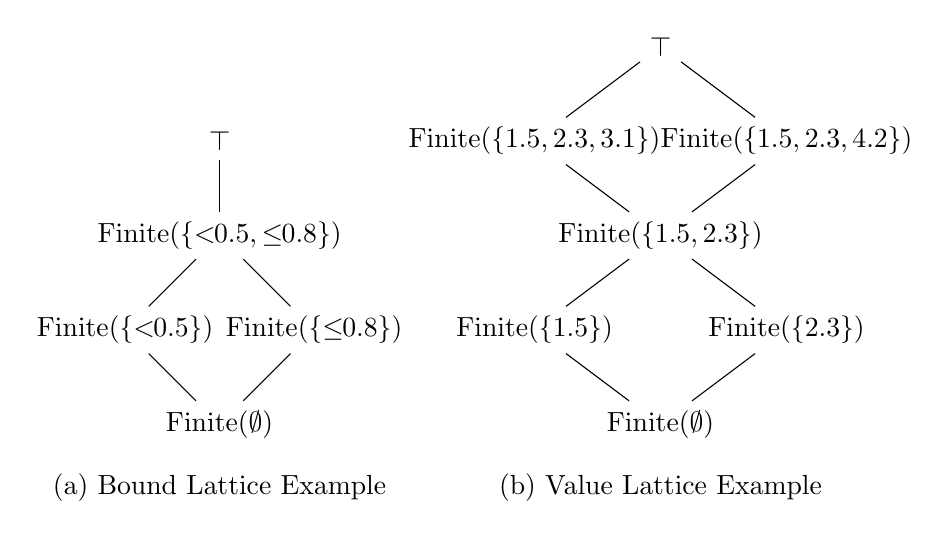
\begin{tikzpicture}[scale=0.8]
  % Individual lattice (left)
  \node (bot1) at (0,0) {$\text{Finite}(\emptyset)$};
  \node (s1) at (-1.5,1.5) {$\text{Finite}(\{<\!\!0.5\})$};
  \node (s2) at (1.5,1.5) {$\text{Finite}(\{\leq\!\!0.8\})$};
  \node (s12) at (0,3) {$\text{Finite}(\{<\!\!0.5, \leq\!\!0.8\})$};
  \node (top1) at (0,4.5) {$\top$};
  
  \draw (bot1) -- (s1);
  \draw (bot1) -- (s2);
  \draw (s1) -- (s12);
  \draw (s2) -- (s12);
  \draw (s12) -- (top1);
  
  \node at (0,-1) {(a) Bound Lattice Example};
  
  % Product lattice (right)
  \node (bot2) at (7,0) {$\text{Finite}(\emptyset)$};
  \node (s3) at (5,1.5) {$\text{Finite}(\{1.5\})$};
  \node (s4) at (9,1.5) {$\text{Finite}(\{2.3\})$};
  \node (s34) at (7,3) {$\text{Finite}(\{1.5, 2.3\})$};
  \node (s5) at (5,4.5) {$\text{Finite}(\{1.5, 2.3, 3.1\})$};
  \node (s6) at (9,4.5) {$\text{Finite}(\{1.5, 2.3, 4.2\})$};
  \node (top2) at (7,6) {$\top$};
  
  \draw (bot2) -- (s3);
  \draw (bot2) -- (s4);
  \draw (s3) -- (s34);
  \draw (s4) -- (s34);
  \draw (s34) -- (s5);
  \draw (s34) -- (s6);
  \draw (s5) -- (top2);
  \draw (s6) -- (top2);
  \node at (7,-1) {(b) Value Lattice Example};
\end{tikzpicture}
\caption{Lattice structure for float types. (a) shows an example bound lattice with comparison bounds. (b) the lattice over real values.}
\label{fig:lattice}
\end{figure}

The typing rules are split into two parts: rules specific to float types and continuous distributions (Figure~\ref{fig:typing-float}), and standard rules for all other language constructs (Figure~\ref{fig:typing-general}).

To understand the float typing rules, it is helpful to understand how discretization works.
A type $\float$[B; V] is discretized as follows:
\begin{itemize}
    \item If $B$ is a finite set of bounds, then the type is discretized to a type $\fin{(n+1)}$ where $n$ is the number of bounds. For instance, if $B = \{<\!\!0.5, \leq\!\!0.8\}$, then the type is discretized to $\fin{3}$, where $\finconst{0}{3}$ represents the range $(-\infty, 0.5)$, $\finconst{1}{3}$ represents the range $[0.5, 0.8]$, and $\finconst{2}{3}$ represents the range $(0.8, \infty)$.
    \item If $B = \top$, then no discretization is performed, and the type remains $\float$.
\end{itemize}

To understand the typing rules, keep in mind that the $B$ set needs to be sufficiently refined (i.e., contain enough comparison points) so that the discretized program has enough information to determine how the original continuous program behaved.

\begin{figure}
\begin{mathpar}
    \inferrule[\textsc{Float-Const}]
    {\ c \in V \text{ or } V = \top}
    {\Gamma \vdash c : \float[B; V]}

    \inferrule[\textsc{Continuous-1}]
    {\ \Gamma \vdash e : \float[B_1; V_1] \text{ and } B_1 \textit{ distinguishes } V_1}
    {\Gamma \vdash \exponential(e) : \float[B; \top]}

    \inferrule[\textsc{Continuous-2}]
    {\ \Gamma \vdash e_1 : \float[B_1; V_1] \text{ and } B_1 \textit{ distinguishes } V_1 \and 
       \Gamma \vdash e_2 : \float[B_2; V_2] \text{ and } B_2 \textit{ distinguishes } V_2}
    {\Gamma \vdash \gaussian(e_1, e_2) : \float[B; \top]}

    \inferrule[\textsc{Less}]
    {\Gamma \vdash e_1 : \float[B; V_1] \and \Gamma \vdash e_2 : \float[B; V_2] \and B \textit{ answers} <\!\!V_2 \text{ or } B \textit{ answers} \leq\!\!V_1}
    {\Gamma \vdash e_1 < e_2 : \bool}

    \inferrule[\textsc{Less-Equal}]
    {\Gamma \vdash e_1 : \float[B; V_1] \and \Gamma \vdash e_2 : \float[B; V_2] \and B \textit{ answers} \leq\!\!V_2 \text{ or } B \textit{ answers} <\!\!V_1}
    {\Gamma \vdash e_1 \leq e_2 : \bool}

\end{mathpar}
\caption{Typing rules for float types and continuous distributions. The notions \emph{distinguishes} and \emph{answers} are defined in Definitions~\ref{def:distinguishes} and \ref{def:answers-less} and \ref{def:answers-less-equal}.}
\label{fig:typing-float}
\end{figure}

\paragraph{Continuous distributions.} Let us first consider the typing rule for single-argument continuous distributions.
The rule states that the argument $\Gamma \vdash e : \float[B; V]$ with the constraint that $B$ distinguishes $V$. The distinguishes predicate is defined as follows:
\begin{definition}
    \label{def:distinguishes}
    $B$ distinguishes $V$ if every interval in $B$ contains at most one value in $V$, or $B = \top$.
\end{definition}
Intuitively $V$ contains the possible values that the float expression can take on, and $B$ distinguishes $V$ if the continuous quantity can be fully recovered by the discretized program.
For example, if $B = \{<\!\!0.5, \leq\!\!0.8\}$ and $V = \{0.2, 0.7\}$, then $B$ distinguishes $V$. The intervals induced by $B$ are $(-\infty, 0.5)$, $[0.5, 0.8]$, and $(0.8, \infty)$. The first interval contains $0.2$, the second contains $0.7$, and the third contains no values from $V$, so the condition holds. In contrast, if $V = \{0.2, 0.3\}$, $B$ would not distinguish $V$ because both values lie in the first interval $(-\infty, 0.5)$.

Note that if $e$ is a constant, then $V = \{e\}$ and $B = \emptyset$ distinguishes $V$ (because $V$ is a singleton set, so there are no two elements that could lie in the same interval).
If $V = \top$ then $V$ essentially contains all possible real values, so we must also have $B = \top$ in that case.

The rule for two-argument continuous distributions is similar, but the argument $\Gamma \vdash e_1 : \float[B_1; V_1]$ and $\Gamma \vdash e_2 : \float[B_2; V_2]$ with the constraint that $B_1$ and $B_2$ distinguish $V_1$ and $V_2$ respectively.



\paragraph{Comparisons.} 
To understand the typing rules for less-than and less-than-or-equal comparisons, let us first consider a comparison $e < c$ where $c$ is a constant and $e$ is a continuously ranging quantity. Intuitively, if $e : \float[B_1; V_1]$ is discretized, then it must still contain enough information to determine whether $e < c$ is true or false. Therefore, $B_1$ must contain the comparison $<\!\!c$.

Similarly, if $c$ is not a literal constant, but has type $c : \float[B_2; V_2]$, then $c$ can take on values in $V_2$. Therefore, if $V = \{v_1, v_2, \dots, v_n\}$ then $B_1$ must contain the comparisons $<\!\!v_1, <\!\!v_2, \dots, <\!\!v_n$. This motivates the following definition:

\begin{definition}
    \label{def:answers-less}
    $B$ answers $<\!\!V$ if $B$ contains comparisons $<\!\!v$ for every $v \in V$, or $B = \top$.
\end{definition}

In the case that $B = \top$, the quantity is not discretized, so the comparison remains continuous.

Lastly, in order to be able to perform the comparison on the discrete values, we insist that $B_1 = B_2$, ensuring that $e$ and $c$ are discretized to the same representation, and $<$ can be discretized to $\finleq{k}$.

It can also be the case that we have a comparison $c < e$ where the continuously ranging quantity $e : \float[B_2; V_2]$ is on the right hand side. In this case, $B_2$ must answer $c\!\!<$, that is, it must contain a comparison $\leq\!\!c$. To make this explicit, consider $2.3 < e$. We can answer this precisely when $B_2$ contains an intervals $(-\infty, 2.3]$ and $(2.3, +\infty)$: the comparison $2.3 < e$ is true if $e$ is in the second interval, and false if $e$ is in the first interval. Of course, it is also ok if $B_2$ is even more precise, as long as it contains the comparison $\leq\!\!2.3$.

\begin{definition}
    \label{def:answers-less-equal}
    $B$ answers $\leq\!\!V$ if $B$ contains comparisons $\leq\!\!v$ for every $v \in V$, or $B = \top$.
\end{definition}

For less-than-or-equal comparisons, the typing rule is similar, but with the conditions reversed.

\begin{figure}
\begin{mathpar}
    \inferrule[\textsc{Var}]
    {\ }
    {\Gamma, x: \tau \vdash x : \tau}

    \inferrule[\textsc{Let}]
    {\Gamma \vdash e_1 : \tau_1 \\
     \Gamma, x: \tau_1 \vdash e_2 : \tau_2}
    {\Gamma \vdash \letkw \; x = e_1 \; \inkw \; e_2 : \tau_2}

    \inferrule[\textsc{If}]
    {\Gamma \vdash e_1 : \bool \\
     \Gamma \vdash e_2 : \tau \\
     \Gamma \vdash e_3 : \tau}
    {\Gamma \vdash \ifkw \; e_1 \; \thenkw \; e_2 \; \elsekw \; e_3 : \tau}

    \inferrule[\textsc{Discrete}]
    {\ }
    {\Gamma \vdash \discrete(p_0, \ldots, p_n) : \fin{n}}

    \inferrule[\textsc{LessEq}]
    {\Gamma \vdash e : \intty}
    {\Gamma \vdash e \leq i : \bool}

    \inferrule[\textsc{Pair}]
    {\Gamma \vdash e_1 : \tau_1 \\
     \Gamma \vdash e_2 : \tau_2}
    {\Gamma \vdash (e_1, e_2) : \tau_1 * \tau_2}

    \inferrule[\textsc{Fst}]
    {\Gamma \vdash e : \tau_1 * \tau_2}
    {\Gamma \vdash \fstkw \; e : \tau_1}

    \inferrule[\textsc{Snd}]
    {\Gamma \vdash e : \tau_1 * \tau_2}
    {\Gamma \vdash \sndkw \; e : \tau_2}

    \inferrule[\textsc{Fun}]
    {\Gamma, x: \tau_1 \vdash e : \tau_2}
    {\Gamma \vdash \funkw \; x \; \rightarrow \; e : \tau_1 \rightarrow \tau_2}

    \inferrule[\textsc{App}]
    {\Gamma \vdash e_1 : \tau_1 \rightarrow \tau_2 \\
     \Gamma \vdash e_2 : \tau_1}
    {\Gamma \vdash e_1 \; e_2 : \tau_2}

    \inferrule[\textsc{True}]
    {\ }
    {\Gamma \vdash \text{true} : \bool}

    \inferrule[\textsc{False}]
    {\ }
    {\Gamma \vdash \text{false} : \bool}

    \inferrule[\textsc{And}]
    {\Gamma \vdash e_1 : \bool \\
     \Gamma \vdash e_2 : \bool}
    {\Gamma \vdash e_1 \logand e_2 : \bool}

    \inferrule[\textsc{Or}]
    {\Gamma \vdash e_1 : \bool \\
     \Gamma \vdash e_2 : \bool}
    {\Gamma \vdash e_1 \logor e_2 : \bool}

    \inferrule[\textsc{Not}]
    {\Gamma \vdash e : \bool}
    {\Gamma \vdash \text{not}\; e : \bool}

    \inferrule[\textsc{Unit}]
    {\ }
    {\Gamma \vdash () : \text{unit}}

    \inferrule[\textsc{FinConst}]
    {0 \leq k < n}
    {\Gamma \vdash \finconst{k}{n} : \fin{n}}

    \inferrule[\textsc{FinLess}]
    {\Gamma \vdash e_1 : \fin{n} \\
     \Gamma \vdash e_2 : \fin{n}}
    {\Gamma \vdash e_1 \finlt{n} e_2 : \bool}

    \inferrule[\textsc{FinLessEq}]
    {\Gamma \vdash e_1 : \fin{n} \\
     \Gamma \vdash e_2 : \fin{n}}
    {\Gamma \vdash e_1 \finleq{n} e_2 : \bool}

    \inferrule[\textsc{Observe}]
    {\Gamma \vdash e : \bool}
    {\Gamma \vdash \text{observe}\; e : \text{unit}}

    \inferrule[\textsc{Seq}]
    {\Gamma \vdash e_1 : \tau_1 \\
     \Gamma \vdash e_2 : \tau_2}
    {\Gamma \vdash e_1; e_2 : \tau_2}

    \inferrule[\textsc{Fix}]
    {\Gamma, f: \tau_1 \rightarrow \tau_2, x: \tau_1 \vdash e : \tau_2}
    {\Gamma \vdash \text{fix}\; f\; x := e : \tau_1 \rightarrow \tau_2}

    \inferrule[\textsc{Nil}]
    {\ }
    {\Gamma \vdash \text{nil} : \text{list}(\tau)}

    \inferrule[\textsc{Cons}]
    {\Gamma \vdash e_1 : \tau \\
     \Gamma \vdash e_2 : \text{list}(\tau)}
    {\Gamma \vdash e_1 :: e_2 : \text{list}(\tau)}

    \inferrule[\textsc{Match}]
    {\Gamma \vdash e : \text{list}(\tau_1) \\
     \Gamma \vdash e_1 : \tau_2 \\
     \Gamma, h: \tau_1, t: \text{list}(\tau_1) \vdash e_2 : \tau_2}
    {\Gamma \vdash \text{match}\; e\; \text{with}\; \text{nil} \rightarrow e_1 \mid h :: t \rightarrow e_2\; \text{end} : \tau_2}

    \inferrule[\textsc{Ref}]
    {\Gamma \vdash e : \tau}
    {\Gamma \vdash \text{ref}\; e : \text{ref}(\tau)}

    \inferrule[\textsc{Deref}]
    {\Gamma \vdash e : \text{ref}(\tau)}
    {\Gamma \vdash !e : \tau}

    \inferrule[\textsc{Assign}]
    {\Gamma \vdash e_1 : \text{ref}(\tau) \\
     \Gamma \vdash e_2 : \tau}
    {\Gamma \vdash e_1 := e_2 : \text{unit}}
\end{mathpar}
\caption{Typing rules for general language constructs}
\label{fig:typing-general}
\end{figure}

The typing rules for the other constructs are standard, and are shown in Figure~\ref{fig:typing-general}.

\paragraph{Subtyping.}
The type system includes a subtyping relation that captures when one type can be safely used in place of another. The subtyping rules are shown in Figure~\ref{fig:subtyping}. For float types $\float[B;V]$, subtyping follows the lattice ordering on $V$: an expression known to range over some set of values can also be considered to range over a superset of those values. For $B$ we require equality to make sure that the discretized representation of the expression cannot be changed by subtyping.

\begin{figure}
\begin{mathpar}
    \inferrule[\textsc{Sub-Refl}]
    {\ }
    {\tau <: \tau}

    \inferrule[\textsc{Sub-Trans}]
    {\tau_1 <: \tau_2 \and \tau_2 <: \tau_3}
    {\tau_1 <: \tau_3}

    \inferrule[\textsc{Sub-Float}]
    {B_1 = B_2 \and V_1 \sqsubseteq V_2}
    {\float[B_1; V_1] <: \float[B_2; V_2]}

    \inferrule[\textsc{Sub-Pair}]
    {\tau_1 <: \tau_1' \and \tau_2 <: \tau_2'}
    {\tau_1 * \tau_2 <: \tau_1' * \tau_2'}

    \inferrule[\textsc{Sub-List}]
    {\tau <: \tau'}
    {\textbf{list}(\tau) <: \textbf{list}(\tau')}

    \inferrule[\textsc{Sub-Arrow}]
    {\tau_1' <: \tau_1 \and \tau_2 <: \tau_2'}
    {\tau_1 \rightarrow \tau_2 <: \tau_1' \rightarrow \tau_2'}

    \inferrule[\textsc{Sub-Type}]
    {\tau_1 <: \tau_2 \and \Gamma \vdash e : \tau_1}
    {\Gamma \vdash e : \tau_2}
\end{mathpar}
\caption{Subtyping relation for Slice types.}
\label{fig:subtyping}
\end{figure}

\section{Type Inference}\label{sec:type-inference}

Type inference for \Slice{} assigns types to every subexpression while simultaneously collecting comparison points that will guide the discretization process. The type system tracks both traditional type information and refinement information specific to floating-point values. The main challenge is that the typing rules are not syntax directed, which we address in this section by using a constraint-based approach.

\paragraph{Overview.}
The inference algorithm performs type checking and constraint generation in a single pass over the AST. For float types $\float[B; V]$, it maintains two separate refinement components:
\begin{itemize}
    \item The \emph{bound bag} $B$ collects comparison bounds (e.g., $<\!\!0.5$, $\leq\!\!1.2$) from sites where the expression is compared
    \item The \emph{value bag} $V$ tracks concrete float constants that flow to the expression
\end{itemize}

Both components start at the bottom of their respective lattices ($\emptyset$) and monotonically accumulate information through constraint propagation. The implementation maintains bags as mutable references with attached listeners that propagate updates immediately when new information becomes available. The listeners of a bag are triggered when the lattice value goes up in the lattice (it can never go down; the changes are always monotone).
For instance, to maintain the constraint $B_1 \leq B_2$, the system registers a listener that propagates updates from $B_1$ to $B_2$ when $B_1$ goes up.

\paragraph{Basic constraints between bags.}
We maintain three types of constraints between bags:
\begin{description}
    \item[Order:] $B_1 \sqsubseteq B_2$ means that $B_1$ is lower than or equal to $B_2$ in the lattice order. This is enforced with a listener on $B_1$ that increases $B_2$ to maintain the constraint.
    \item[Answerability:] $B \textit{ answers} \leq\!\!V$ or $B \textit{ answers} <\!\!V$ means that $B$ contains $\leq\!\!v$ or $<\!\!v$ for every $v \in V$. This is enforced with a listener on $V$ that adds the corresponding bound to $B$.
    \item[Distinguishability:] $B \textit{ distinguishes } V$ means that every interval in $B$ has at most one point in $V$. This is enforced with a listener on $V$ that adds $\leq\!\!v$ to $B$ for every $v \in V$. Note that this may not lead to the coarsest possible bound bag, but it is sound.
\end{description}
In each case, if the bag is set to $\top$, we propagate the required $\top$ to the other bag.

\paragraph{Subtyping constraints between types.}
To maintain subtyping constraints $\tau_1 <: \tau_2$ between types, we recurse into the types according to the rules in \Cref{fig:subtyping}. Whenever one of the sides is a type variable, we instantiate it with the corresponding type of the other side, and add subtyping constraints according to the rules. When both sides are type variables, we add listeners to the type variables that propagate the subtyping constraints whenever one side is instantiated. To enforce equality between types, we enforce subtyping both ways.

\begin{itemize}
    \item \textbf{Base types}: Must match exactly (\bool{}, \intty{}, $\text{fin}(n)$, $\text{unit}$)
    \item \textbf{Float types}: $\float[B_1; V_1] <: \float[B_2; V_2]$ requires:
        \begin{itemize}
            \item $B_1 = B_2$ (bound bags must be equal for safe discretization)
            \item $V_1 \sqsubseteq V_2$ (values flow covariantly)
        \end{itemize}
    \item \textbf{Structural types}: 
        \begin{itemize}
            \item Pairs and lists are covariant in their components
            \item Functions are contravariant in arguments, covariant in results
            \item References are invariant (require exact type match)
        \end{itemize}
\end{itemize}

\paragraph{Type Inference Rules.}
The algorithm traverses the AST, generating types and constraints according to these rules:

\paragraph{Basic Expressions}
\begin{itemize}
    \item Float constants $c$ start with type $\float[\emptyset; \{c\}]$ (empty bounds, singleton value set)
    \item Boolean constants get type \bool{}, finite constants $\finconst{k}{n}$ get type $\text{fin}(n)$
    \item Variables look up their type in the environment
\end{itemize}

\paragraph{Comparisons} 

For a comparison $e_1 < e_2$ (or $e_1 \leq e_2$) we add the appropriate answerability constraints.

\paragraph{Distributions}
\begin{itemize}
    \item Continuous distributions (uniform, gaussian, etc.) get type $\float[\emptyset; \top]$
    \item Parameters' bags are linked according to the distinguishability constraint.
    \item $\discrete(p_0, \ldots, p_n)$ has type $\text{fin}(n+1)$.
\end{itemize}


\paragraph{Other constructs}
Other constructs follow standard typing rules:
\begin{itemize}
    \item $\ifkw \; e_1\; \thenkw \; e_2\; \elsekw \; e_3$: condition must be \bool{}, branches must have unifiable types
    \item $\letkw \; x = e_1 \; \inkw \; e_2$: $x$ gets the type of $e_1$ in the body $e_2$
    \item Sequencing $e_1; e_2$ returns the type of $e_2$, and $e_1$ must have type $\textbf{unit}$.
    \item Pairs, functions, lists, and references follow standard typing rules.
\end{itemize}

\subsection{Algorithm Summary}

The complete type inference creates a new type variable for every subexpression, and establishes constraints between them with a single pass over the AST. The constraints are then solved with the constraint solver, returning an AST where every single expression carries its type. In particular, expressions of type $\float[B; V]$ carry the cut points $B$. The annotated program is ready for discretization, with all comparison points captured in the refinements.

\paragraph{Example.}
Consider the type inference process for this simple program:
\begin{lstlisting}[aboveskip=1em,belowskip=1em,escapechar=!]
    let x = if uniform(0,1) < 0.5 
            then uniform(0,2) 
            else gaussian(0,1) in
    let y = if 1.5 < x
            then 1.8
            else 0.3 in
    x <= y
\end{lstlisting}

The inference proceeds as follows. First, we create a new type variable for every subexpression. Second, the constraint solver finds the types of the subexpressions.
This obtains the following annotated program with unknown bags:

\begin{lstlisting}[aboveskip=1em,belowskip=1em,escapechar=!]
    let x = if (uniform(0,1) : !{\codetype{float[$B_1$; $V_1$]}}!) < (0.5 : !{\codetype{float[$B_2$; $V_2$]}}!)
            then (uniform(0,2) : !{\codetype{float[$B_3$; $V_3$]}}!)
            else (gaussian(0,1) : !{\codetype{float[$B_4$; $V_4$]}}!)
            : !{\codetype{float[$B_x$; $V_x$]}}! in
    let y = if (1.5 : !{\codetype{float[$B_5$; $V_5$]}}!) < (x : !{\codetype{float[$B_x$; $V_x$]}}!)
            then (1.8 : !{\codetype{float[$B_6$; $V_6$]}}!)
            else (0.3 : !{\codetype{float[$B_7$; $V_7$]}}!)
            : !{\codetype{float[$B_y$; $V_y$]}}! in
    (x : !{\codetype{float[$B_x$; $V_x$]}}!) <= (y : !{\codetype{float[$B_y$; $V_y$]}}!)
\end{lstlisting}

The bags are then solved in the following manner:

\begin{enumerate}
    \item \textbf{Initial bags:}
    Float constants get singleton value bags: $V_2=\{0.5\}$, $V_5=\{1.5\}$, $V_6=\{1.8\}$, $V_7=\{0.3\}$.
    Continuous distributions get $\top$ value bags: $V_1=V_3=V_4=\top$.
    All bound bags start empty.

    \item \textbf{Subtyping and equality constraints:}
    The type inference enforces equality on bound bags for subexpressions involved in comparisons or belonging to different branches of an `if` statement.
    \begin{itemize}
        \item From `uniform(0,1) < 0.5`: $B_1 = B_2$.
        \item From the `if` expression assigned to `x`: $B_3 = B_4 = B_x$.
        \item From the `if` expression assigned to `y`: $B_6 = B_7 = B_y$.
        \item From `1.5 < x`: $B_5 = B_x$.
        \item From `x <= y`: $B_x = B_y$.
    \end{itemize}
    All bound bags are therefore in two equivalence classes: $B_{12}$ ($= B_1 = B_2$) and $B_{xy}$ ($=B_x=B_y=B_3=B_4=B_5=B_6=B_7$).

    \item \textbf{Value bag propagation:}
    Value bags are joined at `if` expressions.
    \begin{itemize}
        \item For `x`, $V_x$ is the join of $V_3$ and $V_4$, so $V_x = \top \sqcup \top = \top$.
        \item For `y`, $V_y$ is the join of $V_6$ and $V_7$, so $V_y = \{1.8\} \sqcup \{0.3\} = \{0.3, 1.8\}$.
    \end{itemize}

    \item \textbf{Answerability constraints:}
    Comparisons generate answerability constraints which populate the bound bags.
    \begin{itemize}
        \item `uniform(0,1) < 0.5`: Adds the constraint ``$B_1$ answers $<\!\!V_2$'', which means $B_1$ must contain $<\!0.5$. Since $B_1=B_2$, both become $\{<0.5\}$.
        \item `1.5 < x`: Adds ``$B_x$ answers $< V_5$'', which adds $<\ 1.5$ to $B_x$ (and all bags equal to it).
        \item `x <= y`: Adds ``$B_x$ answers $\leq V_y$'', which adds $\leq\ 0.3$ and $\leq\ 1.8$ to $B_x$.
    \end{itemize}

    \item \textbf{Solution:}
    Combining all constraints on $B_{xy}$ ($=B_x=B_y=B_3=B_4=B_5=B_6=B_7$) gives the final bound bag: $\{ \leq\!0.3, <\!1.5, \leq\!1.8 \}$. The bag $B_{12}$ ($=B_1=B_2$) for the first comparison is $\{ <\!0.5 \}$.
\end{enumerate}

This results in the following fully annotated program:

\begin{lstlisting}[aboveskip=1em,belowskip=1em,escapechar=!]
    let x = if (uniform(0,1) : !{\ft{<0.5}}!) < (0.5 : !{\ftb{<0.5}{0.5}}!)
            then (uniform(0,2) : !{\ft{<=0.3,<1.5,<=1.8}}!)
            else (gaussian(0,1) : !{\ft{<=0.3,<1.5,<=1.8}}!)
            : !{\ft{<=0.3,<1.5,<=1.8}}! in
    let y = if (1.5 : !{\ftb{<=0.3,<1.5,<=1.8}{1.5}}!) < x
            then (1.8 : !{\ftb{<=0.3,<1.5,<=1.8}{1.8}}!)
            else (0.3 : !{\ftb{<=0.3,<1.5,<=1.8}{0.3}}!)
            : !{\ftb{<=0.3,<1.5,<=1.8}{0.3,1.8}}! in
    x <= y
\end{lstlisting}

This example shows how comparison points accumulate in the value and bound bags through the constraint propagation mechanism, even when comparisons appear in different branches of the program.



\section{Discretization}\label{sec:discretization}

After type inference, each float-typed expression carries refinement information in its type $\float[B; V]$. The discretization transformation uses this information to convert continuous probabilistic programs into discrete ones that can be analyzed exactly.

\subsection{Overview}

The discretization process transforms continuous distributions into discrete ones based on the comparison points collected during type inference. The key insight is that if a program only compares a continuous value against certain thresholds, we can partition the continuous range into intervals separated by these thresholds and track only which interval contains the value.

For each expression with type $\float[B; V]$:
\begin{itemize}
    \item If $B = \top$ (unbounded), the expression remains continuous
    \item If $B = \{b_1, \ldots, b_n\}$ (finite bounds), we create $n+1$ intervals
\end{itemize}

\subsection{Discretization Rules}

The transformation $\texttt{discretize}(e)$ is defined recursively on the structure of typed expressions:

\paragraph{Float Constants} For a constant $c$ with type $\float[B; V]$:
\begin{itemize}
    \item If $B = \top$: remains as constant $c$
    \item If $B = \{b_1, \ldots, b_n\}$: becomes $\finconst{k}{n+1}$ where $k$ is the index of the interval containing $c$
\end{itemize}

\paragraph{Continuous Distributions} For a distribution $d$ with type $\float[B; V]$ where $B = \{b_1, \ldots, b_n\}$:
\begin{enumerate}
    \item Extract numeric thresholds $c_1 < \cdots < c_n$ from bounds in $B$
    \item Let $\text{CDF}_d(b_i)$ be the measure of the distribution $d$ on the interval $(-\infty, c_i)$ if $b_i =\ <\!\!c_i$ and on the interval $(-\infty, c_i]$ if $b_i =\ \leq\!\!c_i$. Take $\text{CDF}_d(b_{0}) = 0$ and $\text{CDF}_d(b_{n+1}) = 1$.
    \item Calculate probability mass for each interval using the CDF:
    \[ p_i = \text{CDF}_d(b_i) - \text{CDF}_d(b_{i-1}) \]
    \item Generate $\discrete(p_1, \ldots, p_{n+1})$ returning interval indices.
\end{enumerate}

If $B = \top$, the distribution remains continuous.

\paragraph{Comparisons} For $e_1 < e_2$ where both have type $\float[B; V]$:
\begin{itemize}
    \item If $B = \top$: comparison remains as $\texttt{discretize}(e_1) < \texttt{discretize}(e_2)$
    \item If $B = \{b_1, \ldots, b_n\}$: becomes $\texttt{discretize}(e_1) \finlt{n+1} \texttt{discretize}(e_2)$ (or, $\leq$ becomes $\finleq{n+1}$)
\end{itemize}

The finite comparison $\finlt{n+1}$ operates on interval indices.

\paragraph{Structural Constructs} All other constructs are discretized recursively:
\begin{itemize}
    \item Variables pass through unchanged, though their type may change
    \item Let bindings, conditionals, pairs, etc., recursively discretize subexpressions
\end{itemize}

\paragraph{Effect of discretization on types} The types change as follows:
\begin{itemize}
    \item $\texttt{discretize}(\float[B; V]) = \fin(n+1)$ if $B = \{b_1, \ldots, b_n\}$
    \item $\texttt{discretize}(\float[B; V]) = \float$ if $B = \top$
    \item $\texttt{discretize}(A \to B) = \texttt{discretize}(A) \to \texttt{discretize}(B)$
    \item $\texttt{discretize}(A \times B) = \texttt{discretize}(A) \times \texttt{discretize}(B)$
    \item $\texttt{discretize}(\texttt{list}(A)) = \texttt{list}(\texttt{discretize}(A))$
    \item $\texttt{discretize}(\texttt{ref}(A)) = \texttt{ref}(\texttt{discretize}(A))$
    \item Other types remain unchanged.
\end{itemize}


\subsection{Example}

Consider the following program:
\begin{lstlisting}
let x = uniform(0.0, 1.0) in
if x < 0.5 then 
  if x < 0.7 then 1 else 2
else 3
\end{lstlisting}

After type inference, \texttt{x} has type $\float[\{<0.5, <0.7\}; \top]$. Discretization:
\begin{enumerate}
    \item Extracts thresholds: $\{0.5, 0.7\}$
    \item Creates intervals: $I_0 = (-\infty, 0.5)$, $I_1 = [0.5, 0.7)$, $I_2 = [0.7, \infty)$
    \item Calculates probabilities: $p_0 = 0.5$, $p_1 = 0.2$, $p_2 = 0.3$
    \item Generates: \texttt{let x = discrete(0.5, 0.2, 0.3) in ...}
    \item Transforms comparisons: \texttt{x < 0.5} becomes \texttt{x}$\finlt{3}$\texttt{1}, \texttt{x < 0.7} becomes \texttt{x}$\finlt{3}$\texttt{2}
\end{enumerate}

The discretized program preserves the original semantics while enabling exact inference.

\subsection{Variable Distribution Parameters}

A key challenge arises when distribution parameters are not constant.
For variable distribution parameters, we use the value bag $V$ in $\float[B; V]$ to reconstruct the appropriate distribution to compute the CDF on.
Due to the typing rules, each interval induced by $B$ can contain at most one value from $V$. This means that we can uniquely reconstruct the original floating point number from the interval index, by a series of conditionals.
The distribution can then be discretized as if its parameters were constant in each branch of the conditionals.

Consider the following program:
\begin{lstlisting}
let scale = discrete(0.5, 0.5) in
let x = if scale = 0 then exponential(1.0) 
        else exponential(2.0) in
x < 3.0
\end{lstlisting}

During type inference, the parameter to \texttt{exponential} has type $\float[B_{\text{param}}; \{1.0, 2.0\}]$. The implementation generates runtime dispatch code that:
\begin{enumerate}
    \item Evaluates the parameter expression
    \item Matches against possible constant values from the value bag
    \item Applies appropriate discretization for each case
\end{enumerate}

This ensures correct discretization even when distribution parameters depend on runtime values.




\section{Soundness Proof}\label{sec:soundness}

This section establishes the soundness of our discretization transformation. We proceed in three steps: first, we define a nondeterministic small-step semantics for the base language; second, we extend this to a probabilistic semantics that tracks distributions; and third, we prove that discretization preserves the probabilistic semantics.

\subsection{Nondeterministic Small-Step Semantics}

We begin by defining a small-step operational semantics for \Slice{} that treats probabilistic sampling nondeterministically. This semantics captures the possible values that expressions can take without tracking their probabilities.

\subsubsection{Values}

First, we define the set of values that expressions can evaluate to:
\begin{align*}
v ::= &\; c                                  & \text{float constant} \\
    | &\; \text{true} \mid \text{false}      & \text{boolean value} \\
    | &\; \finconst{k}{n}                    & \text{finite type value} \\
    | &\; i                                  & \text{integer value} \\
    | &\; ()                                 & \text{unit value} \\
    | &\; (v_1, v_2)                         & \text{pair value} \\
    | &\; \funkw \; x \; \rightarrow \; e    & \text{function closure} \\
    | &\; \text{nil}                         & \text{empty list} \\
    | &\; v_1 :: v_2                         & \text{list cons value} \\
    | &\; \ell                               & \text{location (for references)}
\end{align*}

\subsubsection{Evaluation Contexts}

We use evaluation contexts to specify the order of evaluation:
\begin{align*}
E ::= &\; [\cdot] \\
    | &\; \letkw \; x = E \; \inkw \; e \\
    | &\; E < e \mid v < E \\
    | &\; E \leq e \mid v \leq E \\
    | &\; E \finlt{n} e \mid v \finlt{n} E \\
    | &\; E \finleq{n} e \mid v \finleq{n} E \\
    | &\; E \logand e \mid v \logand E \\
    | &\; E \logor e \mid v \logor E \\
    | &\; \text{not}\; E \\
    | &\; \ifkw \; E \; \thenkw \; e_1 \; \elsekw \; e_2 \\
    | &\; (E, e) \mid (v, E) \\
    | &\; \fstkw \; E \mid \sndkw \; E \\
    | &\; E \; e \mid v \; E \\
    | &\; \text{observe}\; E \\
    | &\; E; e \\
    | &\; E :: e \mid v :: E \\
    | &\; \text{match}\; E \; \text{with}\; \ldots \\
    | &\; \text{ref}\; E \\
    | &\; !E \\
    | &\; E := e \mid v := E
\end{align*}

\subsubsection{Small-Step Relation}

We define the small-step relation $e \rightarrow \mathcal{P}(e')$ that maps an expression to a set of possible next expressions. For deterministic constructs, this set is a singleton; for probabilistic sampling, it contains all possible values in the distribution's support.

\paragraph{Basic Rules}

\begin{mathpar}
\inferrule[\textsc{Let}]
{\ }
{\letkw \; x = v \; \inkw \; e \rightarrow \{e[v/x]\}}

\inferrule[\textsc{IfTrue}]
{\ }
{\ifkw \; \text{true} \; \thenkw \; e_1 \; \elsekw \; e_2 \rightarrow \{e_1\}}

\inferrule[\textsc{IfFalse}]
{\ }
{\ifkw \; \text{false} \; \thenkw \; e_1 \; \elsekw \; e_2 \rightarrow \{e_2\}}

\inferrule[\textsc{Fst}]
{\ }
{\fstkw \; (v_1, v_2) \rightarrow \{v_1\}}

\inferrule[\textsc{Snd}]
{\ }
{\sndkw \; (v_1, v_2) \rightarrow \{v_2\}}

\inferrule[\textsc{App}]
{\ }
{(\funkw \; x \; \rightarrow \; e) \; v \rightarrow \{e[v/x]\}}
\end{mathpar}

\paragraph{Comparison Rules}

\begin{mathpar}
\inferrule[\textsc{LessTrue}]
{c_1 < c_2}
{c_1 < c_2 \rightarrow \{\text{true}\}}

\inferrule[\textsc{LessFalse}]
{c_1 \geq c_2}
{c_1 < c_2 \rightarrow \{\text{false}\}}

\inferrule[\textsc{LeqTrue}]
{i_1 \leq i_2}
{i_1 \leq i_2 \rightarrow \{\text{true}\}}

\inferrule[\textsc{LeqFalse}]
{i_1 > i_2}
{i_1 \leq i_2 \rightarrow \{\text{false}\}}
\end{mathpar}

\paragraph{Boolean Operations}

\begin{mathpar}
\inferrule[\textsc{AndTrue}]
{\ }
{\text{true} \logand e \rightarrow \{e\}}

\inferrule[\textsc{AndFalse}]
{\ }
{\text{false} \logand e \rightarrow \{\text{false}\}}

\inferrule[\textsc{OrTrue}]
{\ }
{\text{true} \logor e \rightarrow \{\text{true}\}}

\inferrule[\textsc{OrFalse}]
{\ }
{\text{false} \logor e \rightarrow \{e\}}

\inferrule[\textsc{NotTrue}]
{\ }
{\text{not}\; \text{true} \rightarrow \{\text{false}\}}

\inferrule[\textsc{NotFalse}]
{\ }
{\text{not}\; \text{false} \rightarrow \{\text{true}\}}
\end{mathpar}

\paragraph{List Operations}

\begin{mathpar}
\inferrule[\textsc{MatchNil}]
{\ }
{\text{match}\; \text{nil} \; \text{with}\; \text{nil} \rightarrow e_1 \mid h :: t \rightarrow e_2 \; \text{end} \rightarrow \{e_1\}}

\inferrule[\textsc{MatchCons}]
{\ }
{\text{match}\; v_1 :: v_2 \; \text{with}\; \text{nil} \rightarrow e_1 \mid h :: t \rightarrow e_2 \; \text{end} \rightarrow \{e_2[v_1/h, v_2/t]\}}
\end{mathpar}

\paragraph{Probabilistic Sampling (Nondeterministic)}

For continuous distributions, the small-step relation returns the set of all possible values in the distribution's support:

\begin{mathpar}
\inferrule[\textsc{Uniform}]
{v_1, v_2 \text{ are float values} \\ v_1 < v_2}
{\uniform(v_1, v_2) \rightarrow \{c \mid v_1 \leq c < v_2\}}

\inferrule[\textsc{Gaussian}]
{\mu, \sigma \text{ are float values} \\ \sigma > 0}
{\gaussian(\mu, \sigma) \rightarrow \{c \mid c \in \mathbb{R}\}}

\inferrule[\textsc{Exponential}]
{\lambda \text{ is a float value} \\ \lambda > 0}
{\exponential(\lambda) \rightarrow \{c \mid c \geq 0\}}

\inferrule[\textsc{Beta}]
{\alpha, \beta \text{ are float values} \\ \alpha > 0 \\ \beta > 0}
{\betafn(\alpha, \beta) \rightarrow \{c \mid 0 \leq c \leq 1\}}

\inferrule[\textsc{Discrete}]
{p_0, \ldots, p_n \text{ are probabilities}}
{\discrete(p_0, \ldots, p_n) \rightarrow \{0, 1, \ldots, n\}}
\end{mathpar}

\paragraph{Observations}

\begin{mathpar}
\inferrule[\textsc{ObserveTrue}]
{\ }
{\text{observe}\; \text{true} \rightarrow \{()\}}

\inferrule[\textsc{ObserveFalse}]
{\ }
{\text{observe}\; \text{false} \rightarrow \emptyset}
\end{mathpar}

Note that observing a false condition results in an empty set, representing program termination without producing a value.

\paragraph{References and State}

For references, we extend the semantics with a store $\sigma$ that maps locations to values. The relation becomes $\langle e, \sigma \rangle \rightarrow \mathcal{P}(\langle e', \sigma' \rangle)$:

\begin{mathpar}
\inferrule[\textsc{Ref}]
{\ell \text{ is a fresh location}}
{\langle \text{ref}\; v, \sigma \rangle \rightarrow \{\langle \ell, \sigma[\ell \mapsto v] \rangle\}}

\inferrule[\textsc{Deref}]
{\sigma(\ell) = v}
{\langle !\ell, \sigma \rangle \rightarrow \{\langle v, \sigma \rangle\}}

\inferrule[\textsc{Assign}]
{\ }
{\langle \ell := v, \sigma \rangle \rightarrow \{\langle (), \sigma[\ell \mapsto v] \rangle\}}
\end{mathpar}

\paragraph{Context Rule}

\begin{mathpar}
\inferrule[\textsc{Context}]
{e \rightarrow S}
{E[e] \rightarrow \{E[e'] \mid e' \in S\}}
\end{mathpar}

This nondeterministic semantics captures all possible execution paths of a probabilistic program without tracking the probability of each path. In the next subsection, we will extend this to a probabilistic semantics that properly tracks distributions.

\subsection{Probabilistic Small-Step Semantics}

We now define a probabilistic semantics that tracks the distribution over expressions. Define
%
\[
	\extexprs = \exprs \cup  \{ \error \} \cup \{ \obsfail \}~,
\]
%
and call them \emph{extended expressions}.
%
%where $\error$ indicates a type error and $\obsfail$ denotes observation failure.
The semantic function $\sem{\cdot} \colon \exprs \rightarrow \distexprs$ maps expressions to distributions over expressions, where $\dist{X}$ denotes the space of probability distributions over $X$.

We assume the existence of the Giry monad structure on $\mathcal{D}$, which provides:
\begin{itemize}
    \item $\monunit \colon X \rightarrow \dist{X}$ (also written as $\delta_x$ for the Dirac distribution at $x$)
    \item $\monbind \colon \dist{X} \times (X \to \dist{Y}) \rightarrow \dist{Y}$ (monadic bind)
\end{itemize}

\subsubsection{Deterministic Constructs}

For deterministic constructs, the semantics returns a Dirac distribution:

\paragraph{Values and Basic Operations}
\begin{align*}
\sem{\val} &= \delta_\val \quad \text{(for any value } \val \text{)} \\
\sem{\letkw \; \var = \val \; \inkw \; \expr} &= \delta_{\expr\subst{\val}{\var}} \\
%
%
\sem{ \fstkw \; \val} & = 
\begin{cases}
	\delta_{\val_1}  & \text{if $\val = (\val_1,\val_2)$ for some values $\val_1,\val_2$} \\
	%
	\delta_{\error}  & \text{otherwise}
\end{cases}
%
\\
%
%
\sem{ \sndkw \; \val} & = 
\begin{cases}
	\delta_{\val_2}  & \text{if $\val = (\val_1,\val_2)$ for some values $\val_1,\val_2$} \\
	%
	\delta_{\error}  & \text{otherwise}
\end{cases}
%
\\
%
\sem{ (\funkw \; \var \; \rightarrow \; \expr) \; \val } &= \delta_{\expr\subst{\val}{\var}}\\
\sem{\error} = \delta_\error \\
\sem{\obsfail} = \delta_\obsfail
\end{align*}
%

\paragraph{Conditionals}
\begin{align*}
\sem{ \ifkw \; \val \; \thenkw \; e_1 \; \elsekw \; e_2 } & = 
\begin{cases}
	\sem{\expr_1}  & \text{if $\val = \true$} \\
	%
	\sem{\expr_2}  & \text{if $\val = \false$} \\
	%
	\delta_\error & \text{otherwise}
\end{cases}
\end{align*}
%

\paragraph{Comparisons}
\begin{align*}
\sem{ v_1 < v_2 } &= \begin{cases}
    \delta_{\text{true}} & \text{if $v_1$ and $v_2$ are float constants and~} v_1 < v_2 \\
    \delta_{\text{false}} & \text{if $v_1$ and $v_2$ are float constants and~} v_1 \geq v_2\\
    \delta_\error & \text{otherwise}
\end{cases} \\
\sem{ v_1 \leq v_2 } &=\begin{cases}
	\delta_{\text{true}} & \text{if $v_1$ and $v_2$ are integer values and~} v_1 < v_2 \\
	\delta_{\text{false}} & \text{if $v_1$ and $v_2$ are integer values and~} v_1 \geq v_2\\
	\delta_\error & \text{otherwise}
\end{cases}
\end{align*}
%

\paragraph{Boolean Operations}
\begin{align*}
%\sem{ \text{true} \logand e } &=  \sem{ e } \\
%\sem{ \text{false} \logand e } &= \delta_{\text{false}} \\
%
\sem{ v \logand e } & = \begin{cases}
	\sem{ e } & \text{if $v=\true$} \\
	\delta_{\text{false}} & \text{if $v=\false$} \\
	\delta_\error & \text{otherwise}
\end{cases} \\ 
%
%=
%\sem{ \text{true} \logor e } &= \delta_{\text{true}} \\
%\sem{ \text{false} \logor e } &= \sem{ e } \\
%
\sem{ v \logor e } & = \begin{cases}
	\delta_\true & \text{if $v=\true$} \\
	\sem{ e } & \text{if $v=\false$} \\
	\delta_\error & \text{otherwise}
\end{cases} \\ 
%
%
\sem{ \text{not}\; v } &= 
 \begin{cases}
	\delta_\false & \text{if $v=\true$} \\
	\delta_\true & \text{if $v=\false$} \\
	\delta_\error & \text{otherwise}
\end{cases} \\ 
 \\
%
%\sem{ \text{not}\; \text{true} } &= \delta_{\text{false}} \\
%\sem{ \text{not}\; \text{false} } &= \delta_{\text{true}}
\end{align*}
%


\subsubsection{Compositional Rules}

For compound expressions, we use monadic bind to compose distributions:

\paragraph{Binary Operations}
\begin{align*}
\sem{ e_1 < e_2 } &= \sem{ e_1 } \gg\!= \lambda v_1. \sem{ v_1 < e_2 } \\
\sem{ v_1 < e_2 } &= \sem{ e_2 } \gg\!= \lambda v_2. \sem{ v_1 < v_2 }
\end{align*}

Similar rules apply for $\leq$, $\logand$, $\logor$, and other binary operations.

\paragraph{Let Binding}
\begin{align*}
\sem{ \letkw \; x = e_1 \; \inkw \; e_2 } &= \sem{ e_1 } \gg\!= \lambda v. \sem{ \letkw \; x = v \; \inkw \; e_2 }
\end{align*}

\paragraph{Conditionals}
\begin{align*}
\sem{ \ifkw \; e_1 \; \thenkw \; e_2 \; \elsekw \; e_3 } &= \sem{ e_1 } \gg\!= \lambda v. \sem{ \ifkw \; v \; \thenkw \; e_2 \; \elsekw \; e_3 }
\end{align*}

\paragraph{Function Application}
\begin{align*}
\sem{ e_1 \; e_2 } &= \sem{ e_1 } \gg\!= \lambda v_1. \sem{ v_1 \; e_2 } \\
\sem{ v_1 \; e_2 } &= \sem{ e_2 } \gg\!= \lambda v_2. \sem{ v_1 \; v_2 }
\end{align*}

\paragraph{Pairs and Projections}
\begin{align*}
\sem{ (e_1, e_2) } &= \sem{ e_1 } \gg\!= \lambda v_1. \sem{ (v_1, e_2) } \\
\sem{ (v_1, e_2) } &= \sem{ e_2 } \gg\!= \lambda v_2. \delta_{(v_1, v_2)} \\
\sem{ \fstkw \; e } &= \sem{ e } \gg\!= \lambda v. \sem{ \fstkw \; v } \\
\sem{ \sndkw \; e } &= \sem{ e } \gg\!= \lambda v. \sem{ \sndkw \; v }
\end{align*}

\paragraph{Sequencing}
\begin{align*}
\sem{ e_1; e_2 } &= \sem{ e_1 } \gg\!= \lambda v_1. \sem{ e_2 }
\end{align*}

\paragraph{Finite Type Operations}
\kevin{why don't we distinguish values and compound expressions here?}
\begin{align*}
\sem{ \finconst{k}{n} } &= \delta_{k_{\#n}} \\
%
\sem{ e_1 \finlt{n} e_2 } &= \sem{ e_1 } \gg\!= \lambda v_1. \sem{ v_1 \finlt{n} e_2 } \\
%
\sem{ k_{1,\#n} \finlt{n} k_{2,\#n} } &= \begin{cases}
    \delta_{\text{true}} & \text{if } k_1 < k_2 \\
    \delta_{\text{false}} & \text{otherwise}
\end{cases} \\
%
\sem{ v_1 \finlt{n} v_1 } &= \begin{cases}
	\delta_{\text{true}} & \text{if $v_1 = k_{1,\#n}$ and $v_2=k_{1,\#n}'$ are finite type values and}~k < k' \\
	\delta_{\text{false}} & \text{if $v_1 = k_{1,\#n}$ and $v_2=k_{1,\#n}'$ are finite type values and}~k \geq k' \\
	\delta_{\error} & \text{otherwise}
\end{cases}
\end{align*}

\subsubsection{Probabilistic Distributions}

For sampling expressions, we map to the corresponding probability distributions:
\kevin{double check if type system should ensure the side conditions}

\begin{align*}
\sem{ \uniform(v_1, v_2) } &= \begin{cases}
\text{Uniform}_{[v_1, v_2)}  & \text{if $v_1$ and $v_2$ are float constants with $v_1 < v_2$} \\
%
\delta_\error & \text{otherwise}
\end{cases}
\\
\sem{ \gaussian(v_\mu, v_\sigma) } &= 
 \begin{cases}
	\mathcal{N}(v_\mu, v_\sigma^2)  & \text{if $v_\mu$ and $v_\sigma$ are float constants with $v_\sigma > 0$} \\
	%
	\delta_\error & \text{otherwise}
\end{cases}
\\
\sem{ \exponential(v_\lambda) } &= 
 \begin{cases}
	\text{Exp}(v_\lambda)   & \text{if $v_\lambda$ is a float constant with $v_\lambda > 0$} \\
	%
	\delta_\error & \text{otherwise}
\end{cases}
\\
\sem{ \betafn(v_\alpha, v_\beta) } &= 
 \begin{cases}
	\text{Beta}(v_\alpha, v_\beta)   & \text{if $v_\alpha$ and $v_\beta$ are float constants with $v_\alpha > 0$ and $v_\beta > 0$} \\
	%
	\delta_\error & \text{otherwise}
\end{cases}
\\
\sem{ \discrete(v_0, \ldots, v_n) } &= %\sum_{i=0}^n p_i \cdot \delta_i
\begin{cases}
	\sum_{i=0}^n v_i \cdot \delta_i & \text{if the $v_i$ a are non-negative float constants with $\sum_i v_i = 1$} \\
	%
	\delta_\error  & \text{otherwise}
\end{cases}
\end{align*}
\kevin{double check discrete}

Note that for continuous distributions, we have an implicit coercion from distributions over reals to distributions over constant expressions. That is, if $D$ is a distribution over $\mathbb{R}$, we treat it as a distribution over expressions by mapping each real $r$ to the constant expression $r$.

\subsubsection{Observations}

Observations condition the distribution:

\begin{align*}
\sem{ \text{observe}\; e } &= \sem{ e } \gg\!= \lambda v. \sem{ \text{observe}\; v } \\
%\sem{ \text{observe}\; \text{true} } &= \delta_{()} \\
%\sem{ \text{observe}\; \text{false} } &= \bot
%
\sem{ \text{observe}\; v} &=
\begin{cases}
	\delta_{()}  & \text{if $v=\true$} \\
	%
	\delta_{\obsfail} & \text{if $v=\false$} \\
	%
	\delta_\error & \text{otherwise}
\end{cases}
\end{align*}

where $\bot$ represents the zero measure (failed observation).

\subsubsection{DistrCase}

For distrcase expressions (which represent explicit discrete distributions in the implementation):

\begin{align*}
\sem{ \text{distrcase}\{(e_0, p_0), \ldots, (e_n, p_n)\} } &= \sum_{i=0}^n p_i \cdot \sem{ e_i }
\end{align*}

\subsubsection{Example}

Consider the expression:
\begin{lstlisting}
let x = uniform(0.0, 1.0) in
if x < 0.5 then 1 else 2
\end{lstlisting}

The probabilistic semantics gives:
\begin{align*}
&\sem{ \text{let } x = \uniform(0.0, 1.0) \text{ in if } x < 0.5 \text{ then } 1 \text{ else } 2 } \\
&= \sem{ \uniform(0.0, 1.0) } \gg\!= \lambda x. \sem{ \text{if } x < 0.5 \text{ then } 1 \text{ else } 2 } \\
&= \text{Uniform}_{[0,1)} \gg\!= \lambda x. \sem{ \text{if } x < 0.5 \text{ then } 1 \text{ else } 2 } \\
&= \text{Uniform}_{[0,1)} \gg\!= \lambda x. \begin{cases}
    \delta_1 & \text{if } x < 0.5 \\
    \delta_2 & \text{if } x \geq 0.5
\end{cases} \\
&= 0.5 \cdot \delta_1 + 0.5 \cdot \delta_2
\end{align*}

%This probabilistic semantics forms the foundation for proving that our discretization transformation preserves program behavior.
%%
%\begin{theorem}
%	\label{thm:small-step-well-defined}
%	For every $\expr \in \exprs$, $\sem{\expr}$ is a well defined distribution in $\distextexprs$.
%\end{theorem}
%%
%\begin{proof}
%	By induction on $\exprs$.
%\end{proof}
%
%
\kevin{we will need some relation to nondet semantics. lets see whether we need to add error and obsfail.}
\begin{theorem}
	\label{thm:small-step-well-typed}
	If $\expr : \tau$, then $\sem{\expr}(\{ \error \}) = 0$.
\end{theorem}
%
\begin{proof}
	\kevin{probably} By induction on the derivation tree for $\expr : \tau$.
\end{proof}

\subsection{From Small-Step to Big-Step Semantics}
%


\subsection{Measure Space on Expressions}

To make the probabilistic semantics precise, we need to define an appropriate measure space structure on the set of extended expressions. We construct this measure space using the notion of \emph{expression skeletons}.

\subsubsection{Expression Skeletons}

An expression skeleton is an extended expression with ``holes'' where real-valued constants can appear. Formally, we define:

\begin{definition}[Expression Skeleton]
An expression skeleton $s$ is an extended expression where each occurrence of a float constant is replaced by a hole $\square_i$ for some index $i \in \mathbb{N}$. We denote by $\text{Skel}$ the set of all expression skeletons, and by $\text{holes}(s)$ the number of distinct holes in skeleton $s$.
\end{definition}

For example, the expression $\uniform(0.0, 1.0) < 0.5$ has the skeleton $\uniform(\square_1, \square_2) < \square_3$ with three holes.

\subsubsection{Measure Space Construction}

Given a skeleton $s$ with $n = \text{holes}(s)$ holes, we can instantiate it with a vector $\vec{r} = (r_1, \ldots, r_n) \in \mathbb{R}^n$ to produce a concrete expression $s[\vec{r}]$ by replacing each hole $\square_i$ with the real value $r_i$.

The set of all extended expressions can then be represented as:
\[
\extexprs = \bigsqcup_{s \in \text{Skel}} \{s[\vec{r}] \mid \vec{r} \in \mathbb{R}^{\text{holes}(s)}\}
\]

This is a countable disjoint union because:
\begin{enumerate}
    \item The set of skeletons $\text{Skel}$ is countable (expressions have finite syntax trees)
    \item For each skeleton $s$, the set of instantiations forms a copy of $\mathbb{R}^{\text{holes}(s)}$
    \item Different skeletons produce disjoint sets of expressions
\end{enumerate}

\subsubsection{Measurable Sets}

We equip $\extexprs$ with the $\sigma$-algebra generated by sets of the form:
\[
\{s[\vec{r}] \mid \vec{r} \in B\}
\]
where $s$ is a skeleton and $B \subseteq \mathbb{R}^{\text{holes}(s)}$ is a Borel measurable set.

This construction ensures that:
\begin{itemize}
    \item Basic operations like evaluating an expression to a value are measurable
    \item The distributions returned by our probabilistic semantics are well-defined probability measures
    \item We can integrate over expressions when needed for semantic definitions
\end{itemize}

\subsubsection{Distributions Over Expressions}

When we write $\mathcal{D}(\extexprs)$ in our probabilistic semantics, we mean the space of probability measures on $(\extexprs, \mathcal{F})$ where $\mathcal{F}$ is the $\sigma$-algebra described above.

For continuous distributions like $\uniform(a, b)$, the implicit coercion to $\mathcal{D}(\extexprs)$ works as follows:
\begin{enumerate}
    \item The uniform distribution on $[a, b)$ is a measure on $\mathbb{R}$
    \item We lift it to expressions via the skeleton containing a single hole: $s = \square_1$
    \item The resulting distribution on expressions assigns probability to sets of the form $\{r \mid r \in B\}$ for Borel sets $B \subseteq [a, b)$
\end{enumerate}

This measure-theoretic foundation ensures that our probabilistic semantics is mathematically rigorous and that operations like conditioning (via observations) and marginalization are well-defined. 



\section{Implementation}\label{sec:implementation}

We have implemented \Slice{} as an OCaml-based compiler that transforms continuous probabilistic programs into discrete ones, which can then be analyzed using discrete exact inference engines, leveraging their benefits. At a high-level, our implementation consists of two main components: the \Slice{} compiler (\texttt{slice}) and an off-the-shelf discrete inference engine. Between these two components lies a conversion module that transforms the discretized program specfied in our syntax to a syntax compatible with a discrete inference backend, such as Dice and Roulette which we currently support. Figure~\ref{fig:architecture} shows the overall architecture of the \Slice{} system.

\begin{figure}[h]
\centering
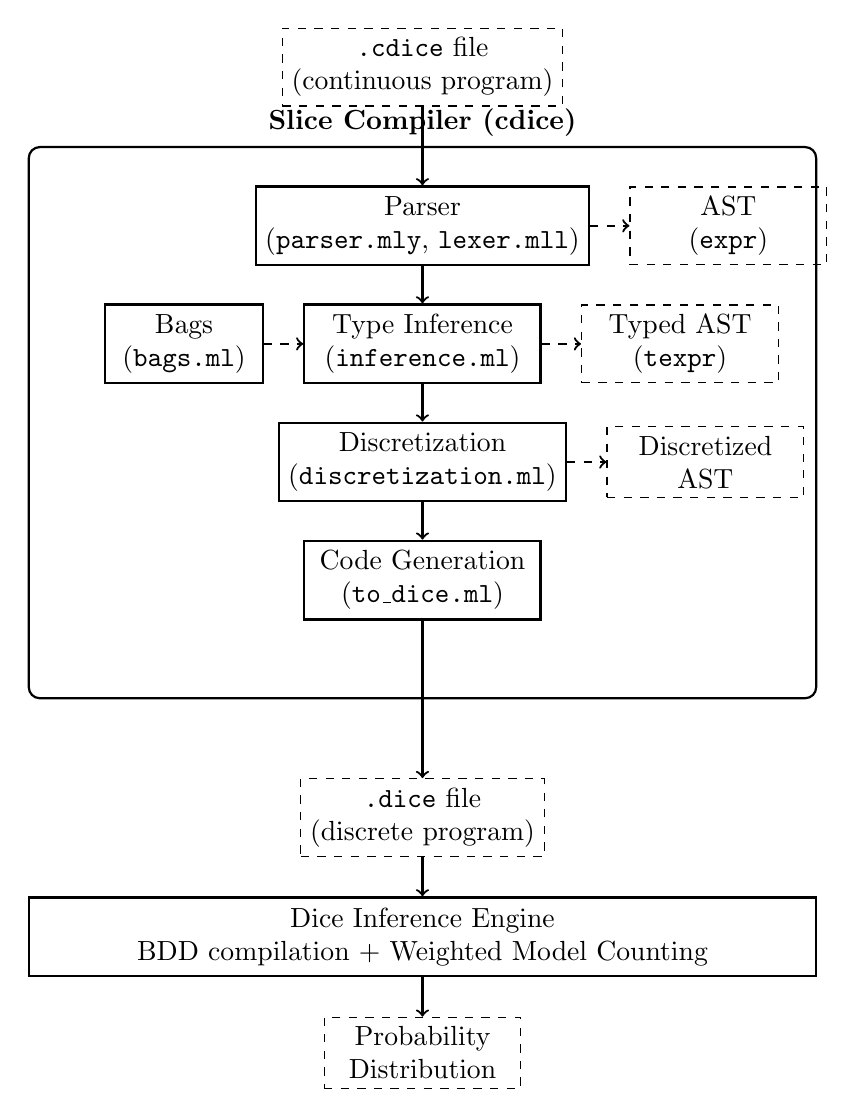
\begin{tikzpicture}[
    node distance=1.5cm,
    component/.style={rectangle, draw, thick, minimum width=3cm, minimum height=1cm, align=center},
    data/.style={rectangle, draw, dashed, minimum width=2.5cm, minimum height=0.8cm, align=center},
    arrow/.style={->, thick},
    bigbox/.style={draw, thick, rounded corners, inner sep=0.3cm}
]
    % Input
    \node[data] (input) {\texttt{.cdice} file\\(continuous program)};
    
    % Slice compiler box
    \node[bigbox, below=0.5cm of input, minimum width=10cm, minimum height=7cm] (slicebox) {};
    \node[above] at (slicebox.north) {\textbf{\Slice{} Compiler (cdice)}};
    
    % Components inside Slice
    \node[component, below=1cm of input] (parser) {Parser\\(\texttt{parser.mly}, \texttt{lexer.mll})};
    \node[component, below of=parser] (typeinf) {Type Inference\\(\texttt{inference.ml})};
    \node[component, below of=typeinf] (disc) {Discretization\\(\texttt{discretization.ml})};
    \node[component, below of=disc] (todice) {Code Generation\\(\texttt{to\_dice.ml})};
    
    % Intermediate data structures
    \node[data, right=0.5cm of parser] (ast) {AST\\(\texttt{expr})};
    \node[data, right=0.5cm of typeinf] (tast) {Typed AST\\(\texttt{texpr})};
    \node[data, right=0.5cm of disc] (dast) {Discretized\\AST};
    
    % Bags module
    \node[component, left=0.5cm of typeinf, minimum width=2cm] (bags) {Bags\\(\texttt{bags.ml})};
    
    % Output from Slice
    \node[data, below=1cm of slicebox] (dice) {\texttt{.dice} file\\(discrete program)};
    
    % Dice engine
    \node[component, below=0.5cm of dice, minimum width=10cm] (diceengine) {Dice Inference Engine\\BDD compilation + Weighted Model Counting};
    
    % Final output
    \node[data, below=0.5cm of diceengine] (output) {Probability\\Distribution};
    
    % Arrows
    \draw[arrow] (input) -- (parser);
    \draw[arrow] (parser) -- (typeinf);
    \draw[arrow] (typeinf) -- (disc);
    \draw[arrow] (disc) -- (todice);
    \draw[arrow] (todice) -- (dice);
    \draw[arrow] (dice) -- (diceengine);
    \draw[arrow] (diceengine) -- (output);
    
    % Side arrows for data structures
    \draw[arrow, dashed] (parser) -- (ast);
    \draw[arrow, dashed] (typeinf) -- (tast);
    \draw[arrow, dashed] (disc) -- (dast);
    \draw[arrow, dashed] (bags) -- (typeinf);
\end{tikzpicture}
\caption{Architecture of the \Slice{} system. The \Slice{} compiler transforms continuous probabilistic programs into discrete ones through type-directed discretization. The resulting discrete program is then processed by the Dice inference engine to compute exact probability distributions.}
\label{fig:architecture}
\end{figure}

\subsection{Implementation Details}

\paragraph{Parser and Lexer} The frontend uses OCaml's Menhir parser generator to parse \texttt{.slice} source files. The parser (\texttt{parser.mly}) defines the concrete syntax and produces an abstract syntax tree (AST) represented by the \texttt{expr} type. The lexer (\texttt{lexer.mll}) handles tokenization, including special tokens for finite type comparisons (e.g., \texttt{<\#n}).

\paragraph{Type Inference} The type inference module (\texttt{inference.ml}) implements the two-bag type system described in Section~\ref{sec:type-inference}. It uses a constraint-based approach with unification to infer types while collecting comparison bounds. The implementation features:
\begin{itemize}
    \item A union-find data structure for managing bags efficiently
    \item Listener patterns for propagating constraints between related expressions
    \item Subtyping rules that ensure proper information flow
\end{itemize}

\paragraph{Bags Module} The \texttt{bags.ml} module provides the lattice-based data structures for tracking bounds and values. It implements:
\begin{itemize}
    \item Generic bag operations (union, equality checking)
    \item Specialized \texttt{BoundBag} for comparison bounds ($<c$, $\leq c$)
    \item \texttt{FloatBag} for tracking concrete float values
    \item Efficient representation using either finite sets or $\top$
\end{itemize}

\paragraph{Discretization} The discretization module (\texttt{discretization.ml}) transforms typed continuous programs into discrete ones. For each continuous distribution, it:
\begin{enumerate}
    \item Extracts comparison thresholds from the bound bag
    \item Computes interval probabilities using distribution CDFs
    \item Generates equivalent discrete distributions
    \item Transforms comparisons to operate on interval indices
\end{enumerate}

\paragraph{Code Generation} The \texttt{to\_dice.ml} and \texttt{to\_roulette.ml} module generates Dice and Roulette source code from the discretized AST, respectively. It handles the translation of \Slice{} constructs to their Dice and Roulette equivalents, including special handling for finite types that become integers in Dice.

\paragraph{Runtime and Evaluation} The implementation includes:
\begin{itemize}
    \item An interpreter (\texttt{interp.ml}) for sampling-based execution
    \item Statistical testing to verify discretization correctness
    \item Support for multiple output formats (Dice, SPPL)
\end{itemize}

\subsection{Integration with Backends}
We currently allow \Slice{} to be compatible to two different discrete inference engines: Dice provides exact inference for discrete probabilistic programs using binary decision diagrams (BDDs) and weighted model counting, and Roulette provides exact inference for discrete programs using an SMT solver with the aim of providing more expressivity. To work seamlessly with Dice, \Slice{} successfully maps 1) discrete distributions to Dice's \texttt{discrete} construct, 2) finite types to bounded integers of the form \texttt{int(size, value)}, and 3) observations to Dice's conditioning primitives. To work seamlessly with Roulette, \Slice{} successfully maps 1) discrete distributions to a chain of if-else statements with \texttt{flip}s, as Roulette currently does not support such a \texttt{discrete} construct, and 2) data structures, higher order functions, recursion, and mutable state as was previously unsupported by Dice to their Roulette counterparts. Finally, tying everything together is the \texttt{slice.py} script that automates the complete workflow, piping the output of \Slice{} directly to Dice or Roulette for inference.

% Listings setup
\lstset{
  basicstyle=\scriptsize\ttfamily,
  breaklines=true,
  columns=fullflexible,
  frame=none,
  backgroundcolor=\color{gray!5},
  showstringspaces=false
}

% Saveboxes for code blocks
\newsavebox{\boxone}
\begin{lrbox}{\boxone}
\begin{minipage}{5.2cm}
\begin{lstlisting}
let g = gaussian(0, 1) in
let check = g < 0.1 in
let x = if check then
    uniform(0, 0.2)
  else
    uniform(0.8, 1.0) in
x < 0.15
\end{lstlisting}
\end{minipage}
\end{lrbox}

\newsavebox{\boxtwo}
\begin{lrbox}{\boxtwo}
\begin{minipage}{5.2cm}
\begin{lstlisting}
let g = discrete(0.539828: 0#2, 0.460172: 1#2) in
let check = g <#2 1#2 in
  let x = if check then
        discrete(0.75: 0#2, 0.25: 1#2)
      else
        discrete(0: 0#2, 1: 1#2) in
    x <#2 1#2
\end{lstlisting}
\end{minipage}
\end{lrbox}

\newsavebox{\boxthree}
\begin{lrbox}{\boxthree}
\begin{minipage}{5.2cm}
\begin{lstlisting}
let g = discrete(0.539828, 0.460172) in
let check = g < int(1,1) in
  let x = if check then
        discrete(0.75, 0.25)
      else
        discrete(0., 1.) in
    x < int(1,1)
\end{lstlisting}
\end{minipage}
\end{lrbox}

\newsavebox{\boxfour}
\begin{lrbox}{\boxfour}
\begin{minipage}{5.2cm}
\begin{lstlisting}
(define g (if (flip 0.539828) 0 1))
(define check (< g 1))
(define x (if check 
               (if (flip 0.75) 0 1) 
               (if (flip 0.0) 0 1)))
(< x 1)
\end{lstlisting}
\end{minipage}
\end{lrbox}


\begin{center}
\begin{tikzpicture}[
    box/.style={
    draw,
    thick,
    align=left,
    inner sep=4pt,
    minimum width=5.4cm,
    minimum height=2.5cm
    },
    arrow/.style={
    -{Latex[length=2.5mm]},
    thick
    }
]

    % Top row
    \node[box] (box1) {\usebox{\boxone}};
    \node[box, right=1.6cm of box1] (box2) {\usebox{\boxtwo}};

    % Bottom row: tightly packed under box2
    \coordinate (belowcenter) at ($(box2.south) + (0,-2.2cm)$);
    \node[box, anchor=north east] (box3) at ($(belowcenter) + (-2.0cm, 0)$) {\usebox{\boxthree}};
    \node[box, anchor=north west] (box4) at ($(belowcenter) + (-1.0cm, 0)$) {\usebox{\boxfour}};

    % Arrows
    \draw[arrow] (box1) -- (box2);
    \draw[arrow] (box2.south) -- (box3.north);
    \draw[arrow] (box2.south) -- (box4.north);

\end{tikzpicture}
\end{center}

\subsection{Engineering Considerations}

The implementation prioritizes correctness and clarity:
\begin{itemize}
    \item Extensive use of OCaml's type system for safety
    \item Modular design allowing independent testing of components
    \item Clear separation between syntax-directed and semantic phases
    \item Comprehensive test suite including adversarial examples
\end{itemize}

The \Slice{} compiler consists of approximately 3,400 lines of OCaml code (including the lexer, parser, type inference engine, discretization engine, and code generator), demonstrating that powerful program transformations can be implemented concisely.

The system is open-source and available at \url{https://github.com/[repository-url]}, along with benchmarks and documentation.




\section{Evaluation}\label{sec:evaluation}
This section confirms that the performance of \Slice{} is competitive with existing state-of-the-art exact and approximate inference solvers. In particular, we evaluate \Slice{} against SPPL~\cite{Saad2021SPPL}, an exact inference solver for continuous programs, and HyBit, an approximate inference solver for continuous programs. The evaluation consists of three sets of programs. First is a series of synthetic benchmarks designed to test the asymptotic scaling of our system against SPPL. Second is a set of benchmarks for verifying fairness properties of decision trees, as characterizing the fairness of classification algorithms is an interesting application area of probabilistic programs in machine learning. Lastly, we evaluate \Slice{} on a series of small baseline programs commonly used to test PPLs in the literature. 

\subsection{Experimental Setup}\label{sec:experimenal-setup}
All experiments were run on a ..., using the original version of Dice (2020) from Holtzen et. al.~\cite{Holtzen2020Dice}. Each experiment was carried out using a consistent-effort approach, with the goal of determining the most effective encoding for the program in each language and making sure that programs were equivalent across all systems. 

\subsection{Synthetic benchmarks}\label{sec:synthetic-benchmarks}
To evaluate the asymptotic performance of \Slice{}, we designed seven synthetic benchmarks that stress-test different aspects of probabilistic programs with continuous distributions. Each benchmark generates programs that grow linearly in size in the number of comparison tests (e.g. number of $<$ operators) to measure how execution time scales. This bears resemblence to how scalability is tested for discrete PPLs in the litearture: by growing the program by adding one additional layer to the chain of \texttt{flips} that depends on the previous. Doing so results in a path enumeration that grows exponentially in the number of layers. We generate programs of varying structure:

\subsubsection{Conditional Independence.} 
If a variable \texttt{z} is conditionally independent of \texttt{x} given \texttt{y}, then \texttt{y} acts as a kind of interface between \texttt{x} and \texttt{z} that allows inference to be split into two separate analyses. Bayesian networks use conditional independence to compactly represent complex distributions, and these independence relationships capture essential structure in many real-world applications. We test programs where each variable's distribution depends on comparisons with previous variables, specifically when:

\begin{itemize}
\item Each variable depends on its immediate predecessor through conditional statements. This creates a chain of dependencies where $x_i$ depends on whether $x_{i-1} < c$ for some constant $c$. See Figure~\ref{fig:cond-benchmarks-a}.
\item Each variable depends on a randomly chosen previous variable through conditional statements. This creates a more complex dependency graph, a chain of dependencies where $x_i$ depends on whether $x_1, ..., x_{i-1}$ chosen uniformly at random is $< c$ for some constant $c$. See Figures~\ref{fig:cond-benchmarks-b} and~\ref{fig:cond-benchmarks-c}.
\end{itemize}

\begin{figure}[!t]
\centering
\begin{subfigure}{0.32\textwidth}
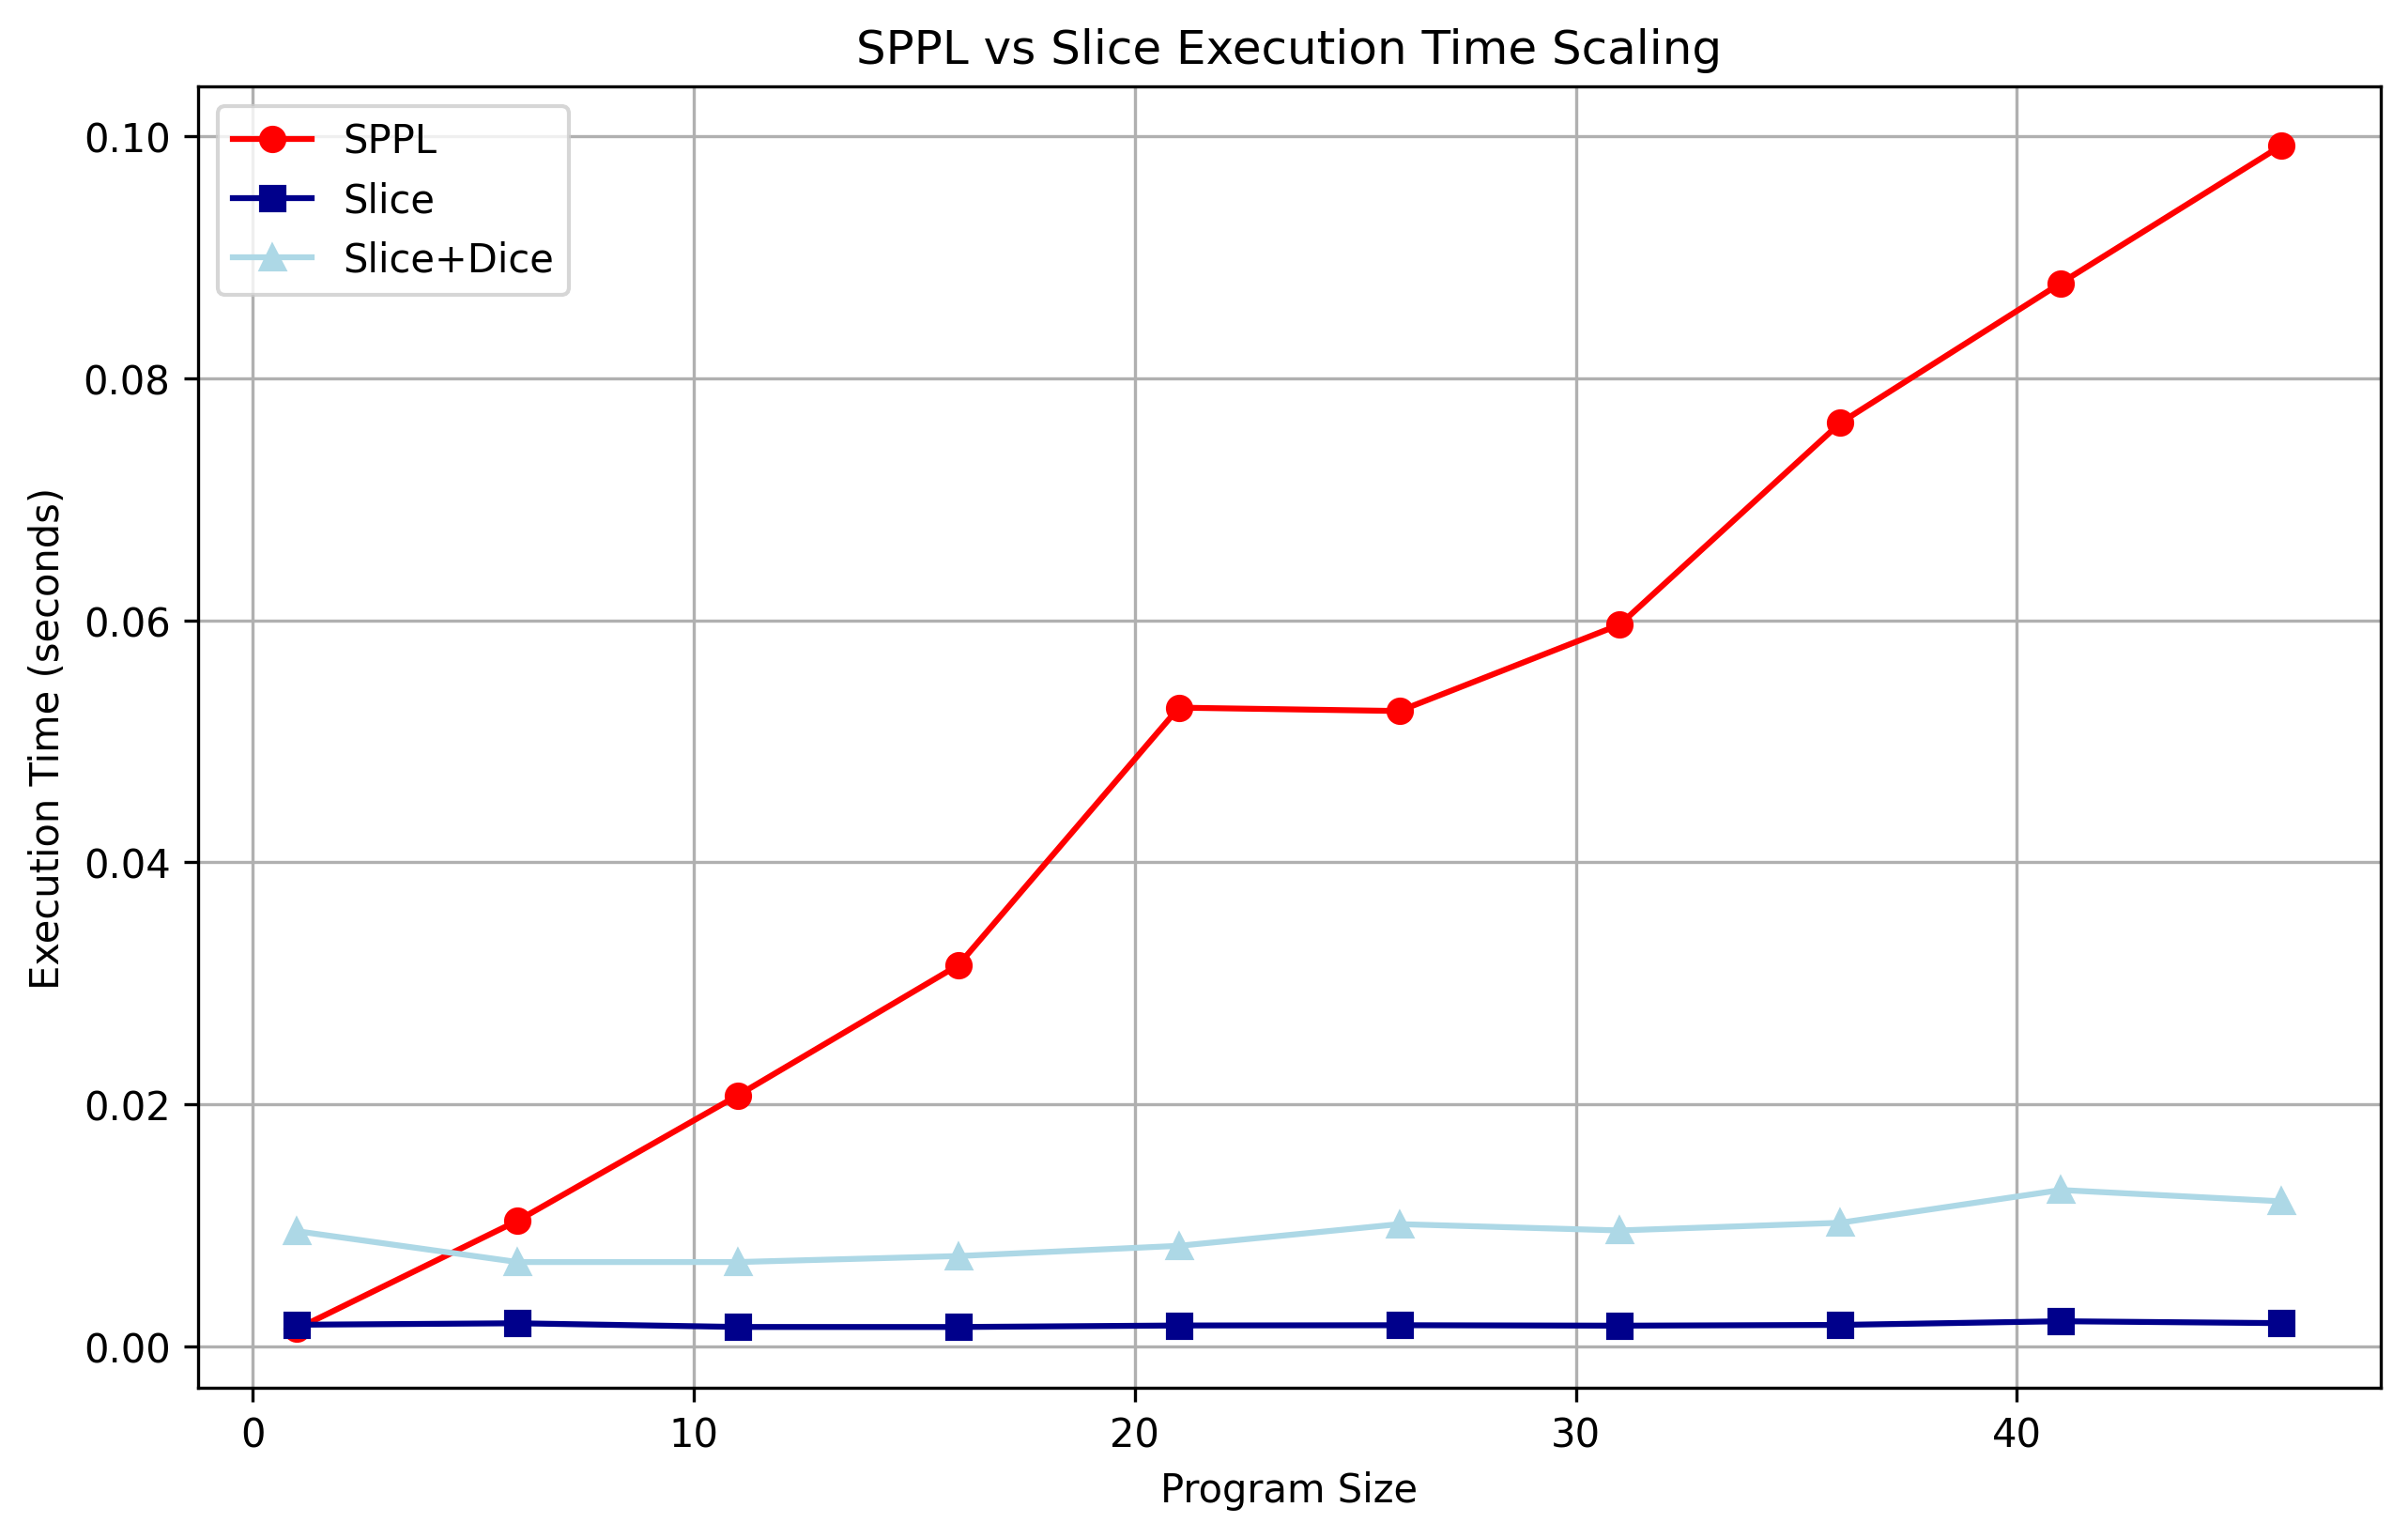
\includegraphics[width=\textwidth]{../images/scaling/build_conditional_independent_slice.png}
\caption{Conditional Independent}
\label{fig:cond-benchmarks-a}
\end{subfigure}
\hfill
\begin{subfigure}{0.32\textwidth}
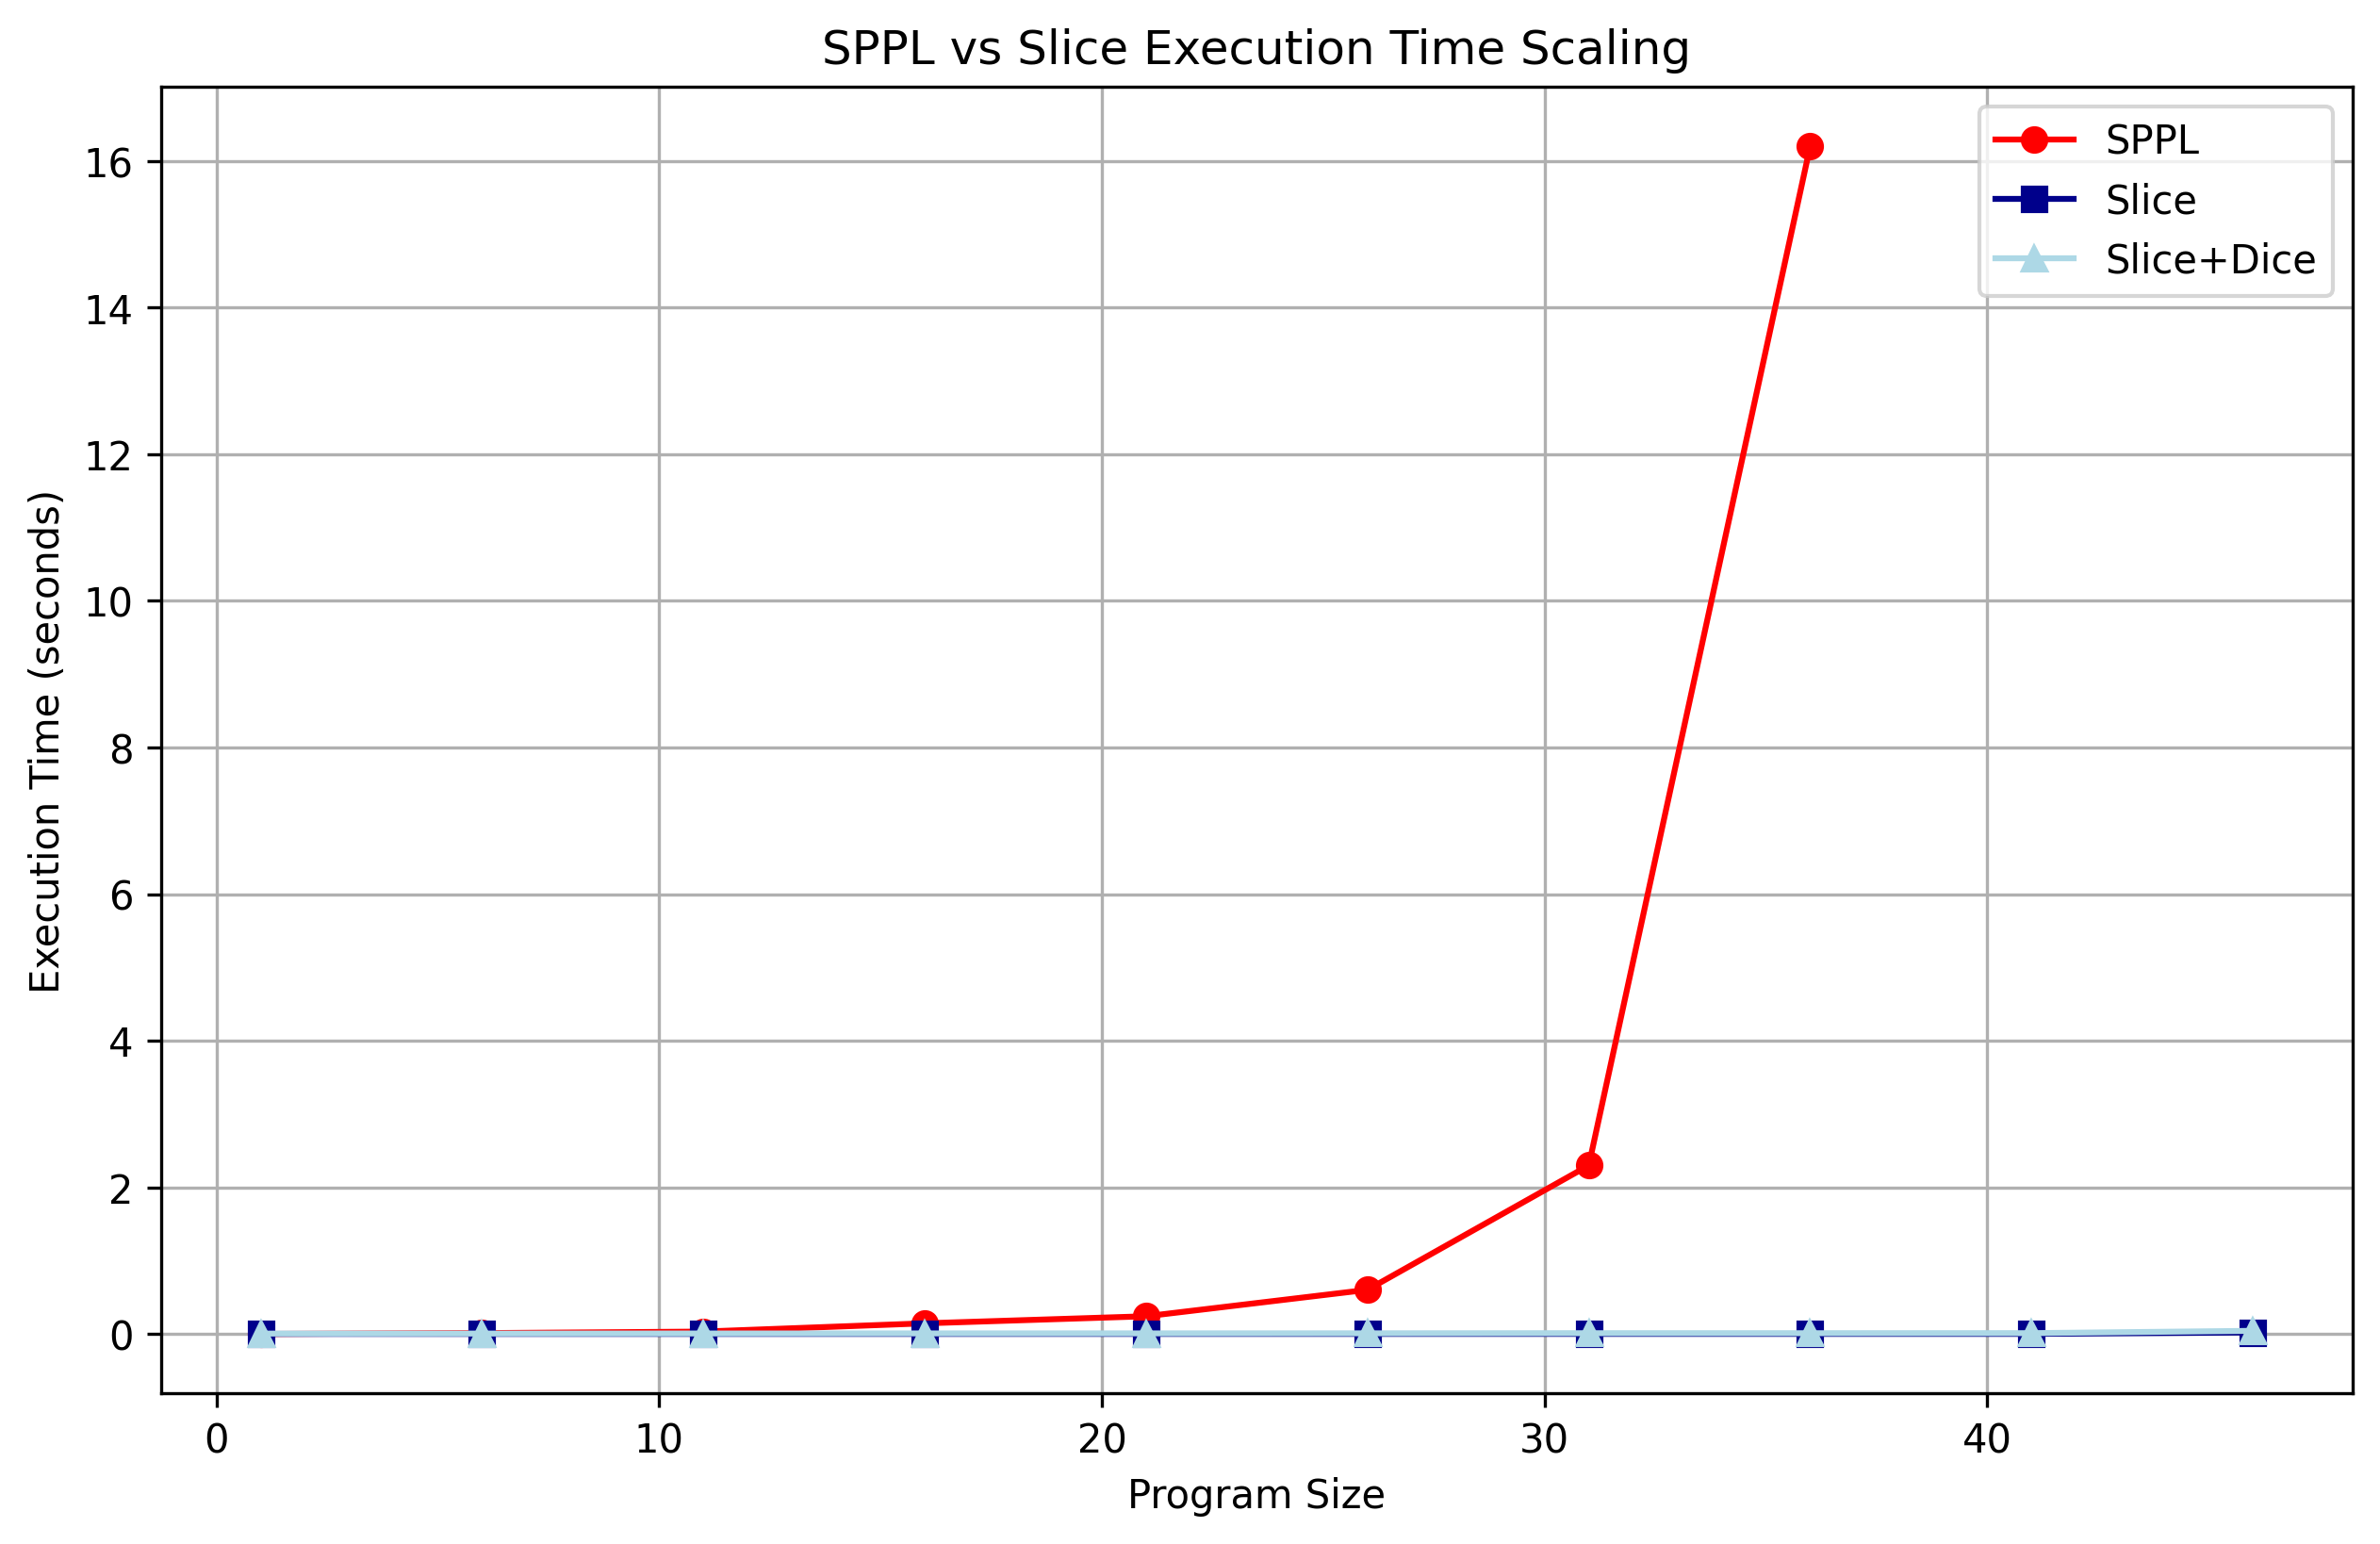
\includegraphics[width=\textwidth]{../images/scaling/build_conditional_random_independent_slice_1.png}
\caption{Conditional Random 1}
\label{fig:cond-benchmarks-b}
\end{subfigure}
\hfill
\begin{subfigure}{0.32\textwidth}
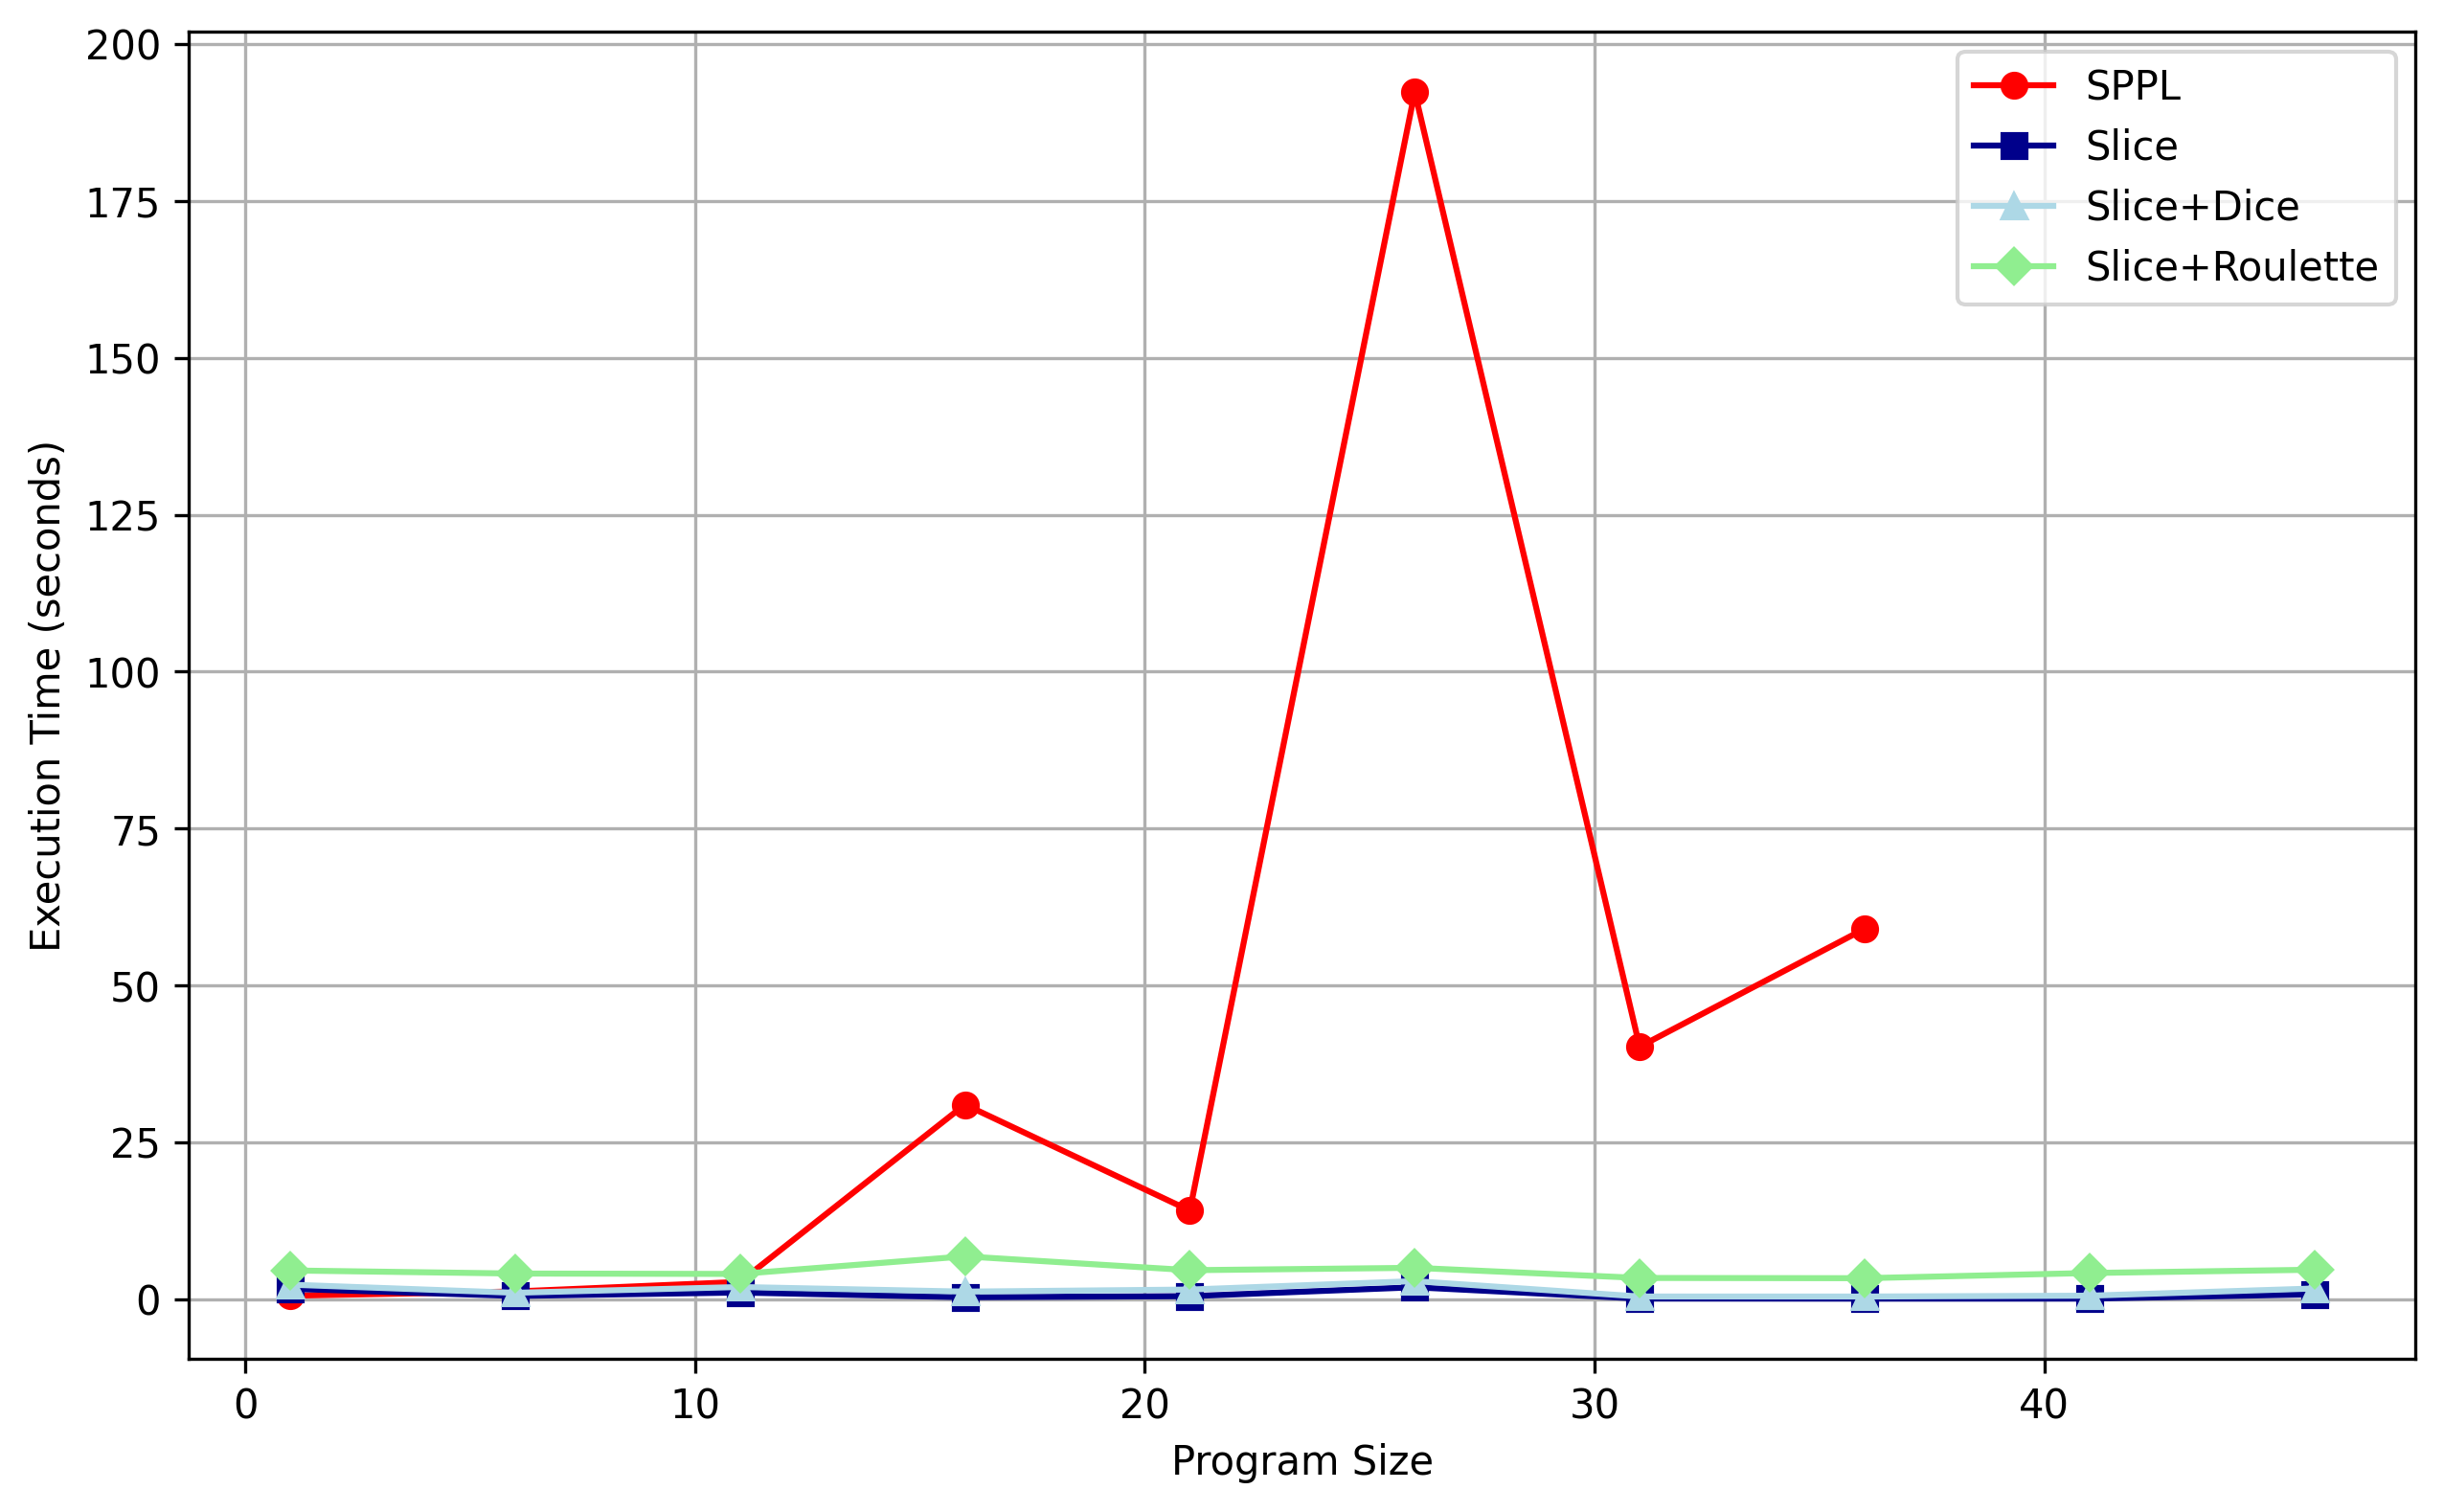
\includegraphics[width=\textwidth]{../images/scaling/build_conditional_random_independent_slice_2.png}
\caption{Conditional Random 2}
\label{fig:cond-benchmarks-c}
\end{subfigure}
\caption{Scaling results for conditional independence benchmarks. SPPL (red) shows exponential growth and times out early, while Slice (blue), Slice+Dice (light blue), and Slice+Roulette (light green) maintain near-linear scaling.}
\label{fig:cond-benchmarks}
\end{figure}

\subsubsection{Alternating Guards.}
We test programs with alternating comparison patterns,
where the control flow depends on earlier random variables. This pattern is characteristic of hierarchical or history-dependent probabilistic systems. Specifically, we test when:

\begin{itemize}
\item Variables in conditionals alternate based on a guard span parameter. For example, with span 3, guards cycle through $x_1, x_2, x_3, x_1, x_2, x_3, ...$ See Figure~\ref{fig:alt-benchmarks-a}. This may lead to many unused code fragments, however. This led us to generate programs whose if-else bodies depend on the immediate predecessor variable. See Figures~\ref{fig:alt-benchmarks-b} and~\ref{fig:alt-benchmarks-c}.

\item Variables in conditionals alternate based on a guard span parameter, but we add randomization in the selection of continuous distributions in the if-else bodies. See Figure~\ref{fig:alt-benchmarks-d}.
\end{itemize}

\begin{figure}[!t]
\centering
\begin{subfigure}{0.48\textwidth}
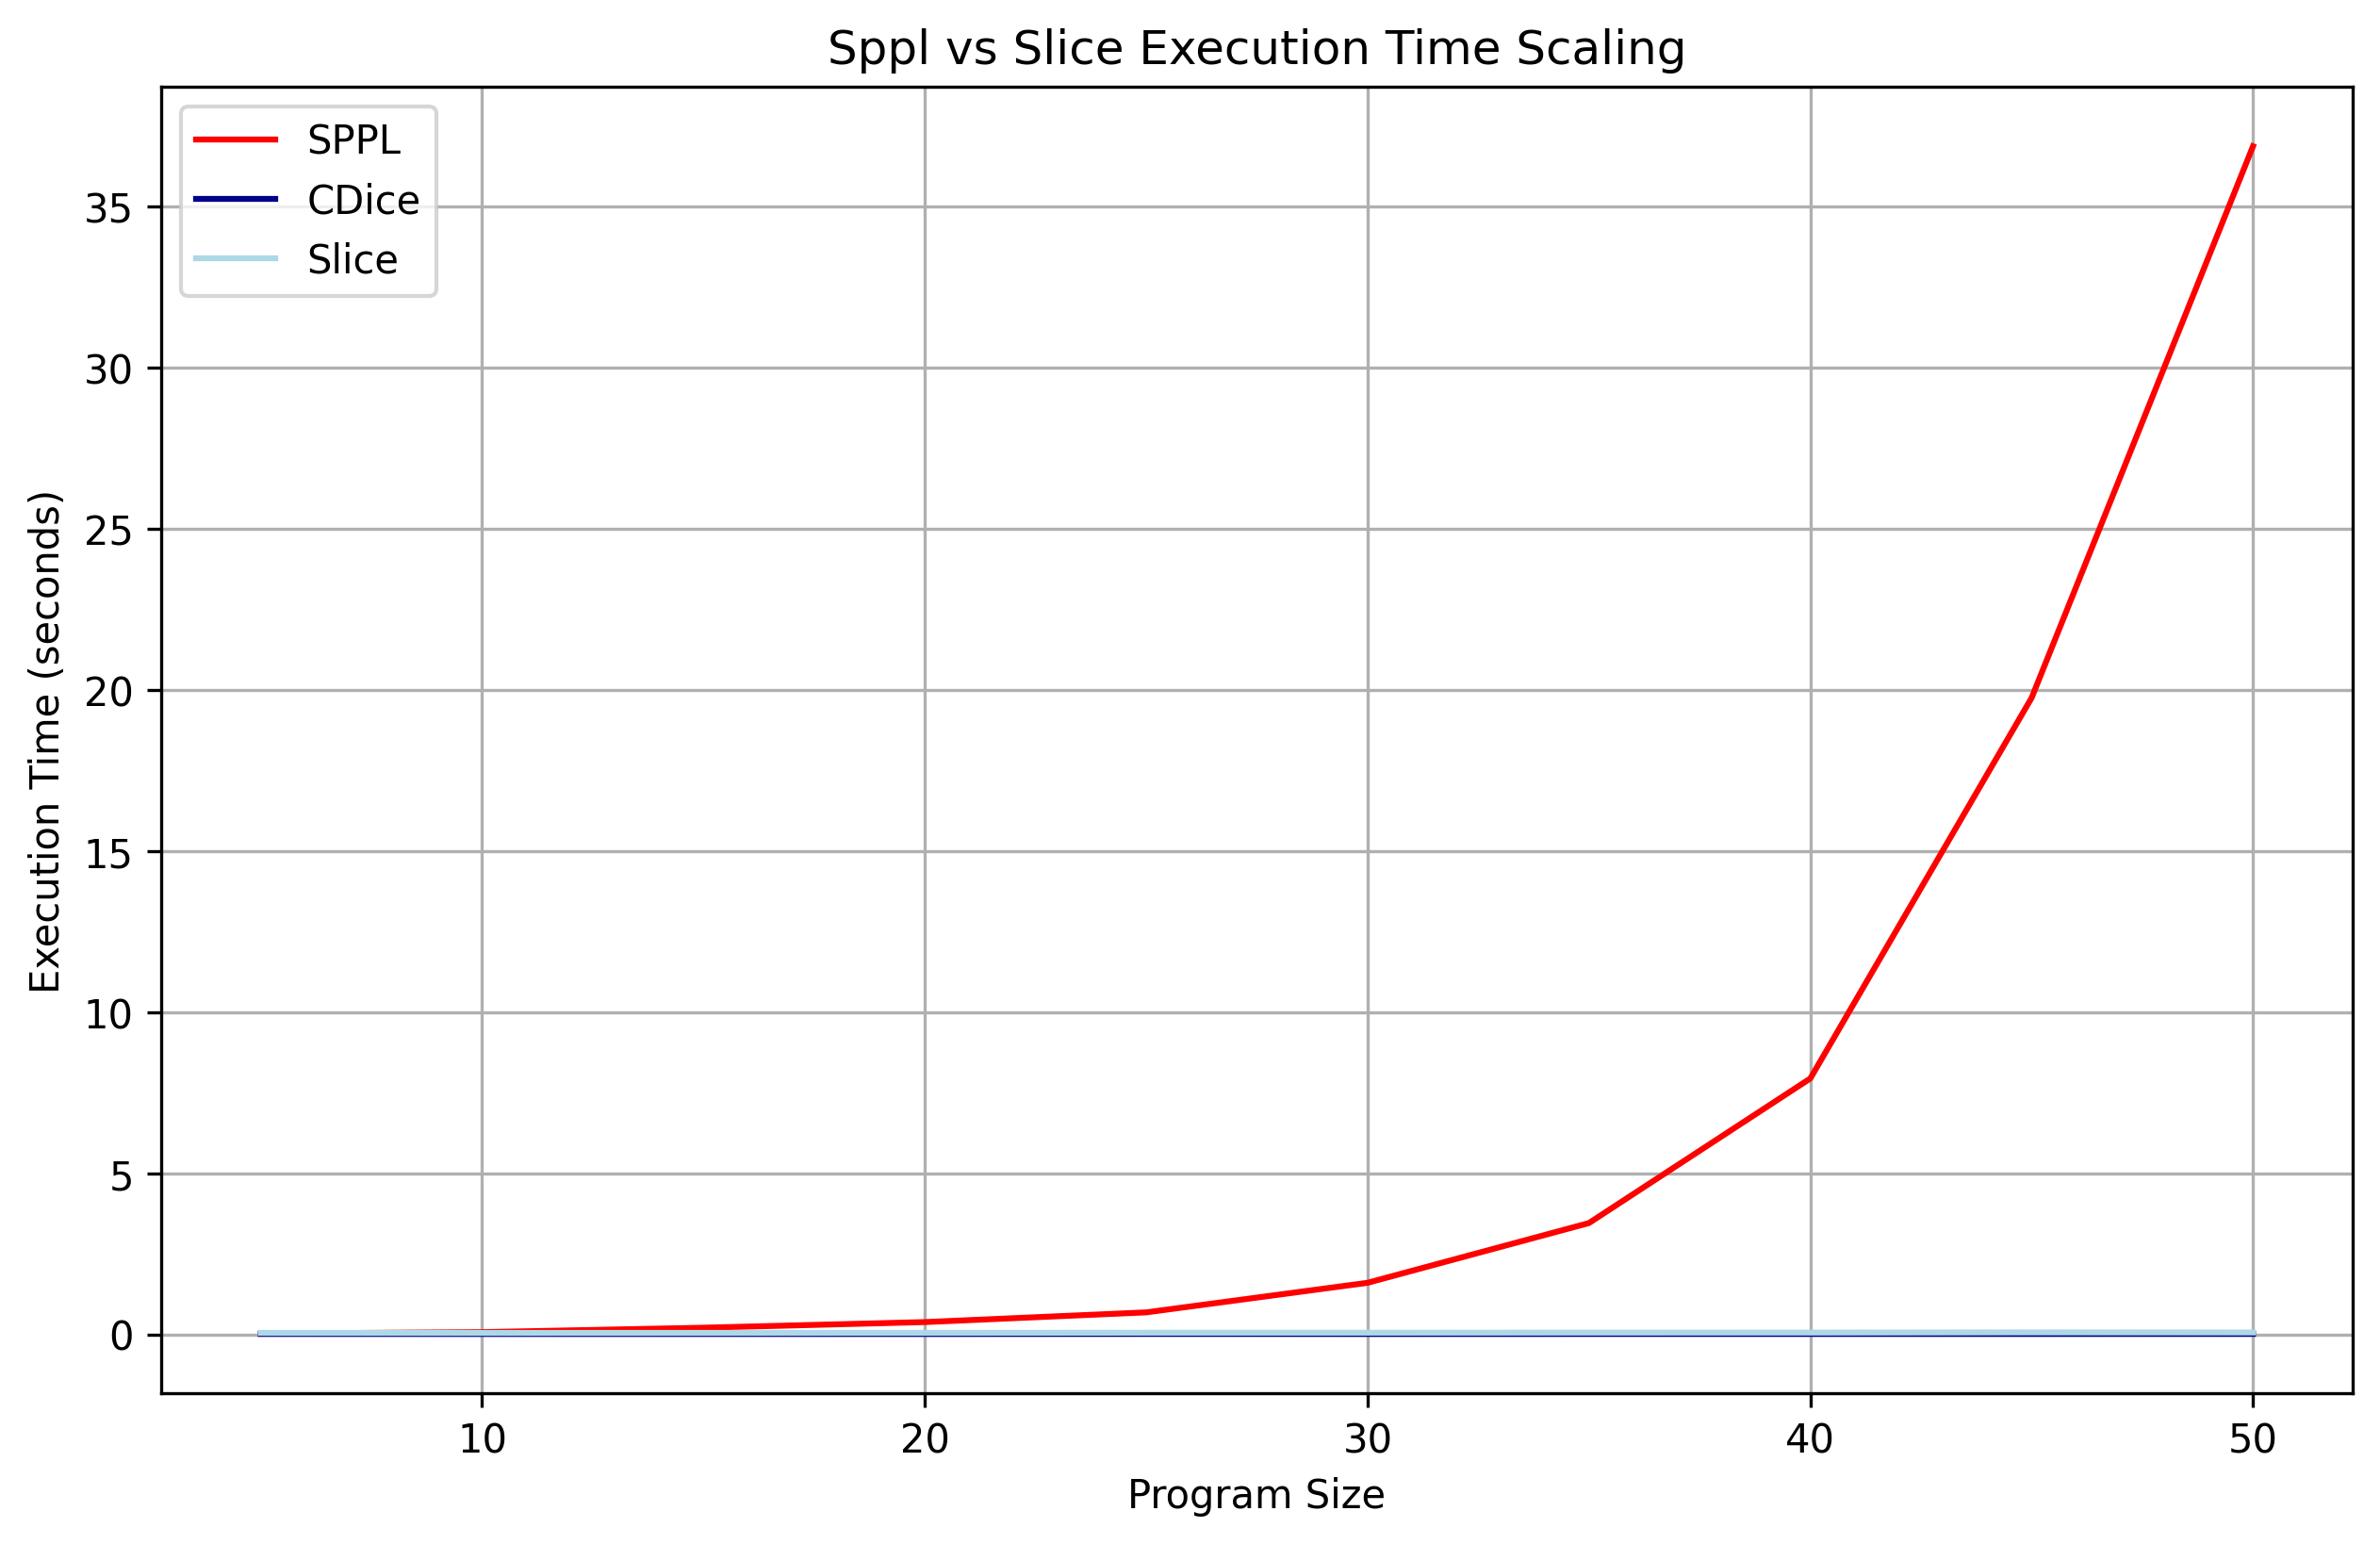
\includegraphics[width=\textwidth]{../images/scaling/build_alternating_guard_contdice_1.png}
\caption{Alternating Guard 1}
\label{fig:alt-benchmarks-a}
\end{subfigure}
\hfill
\begin{subfigure}{0.48\textwidth}
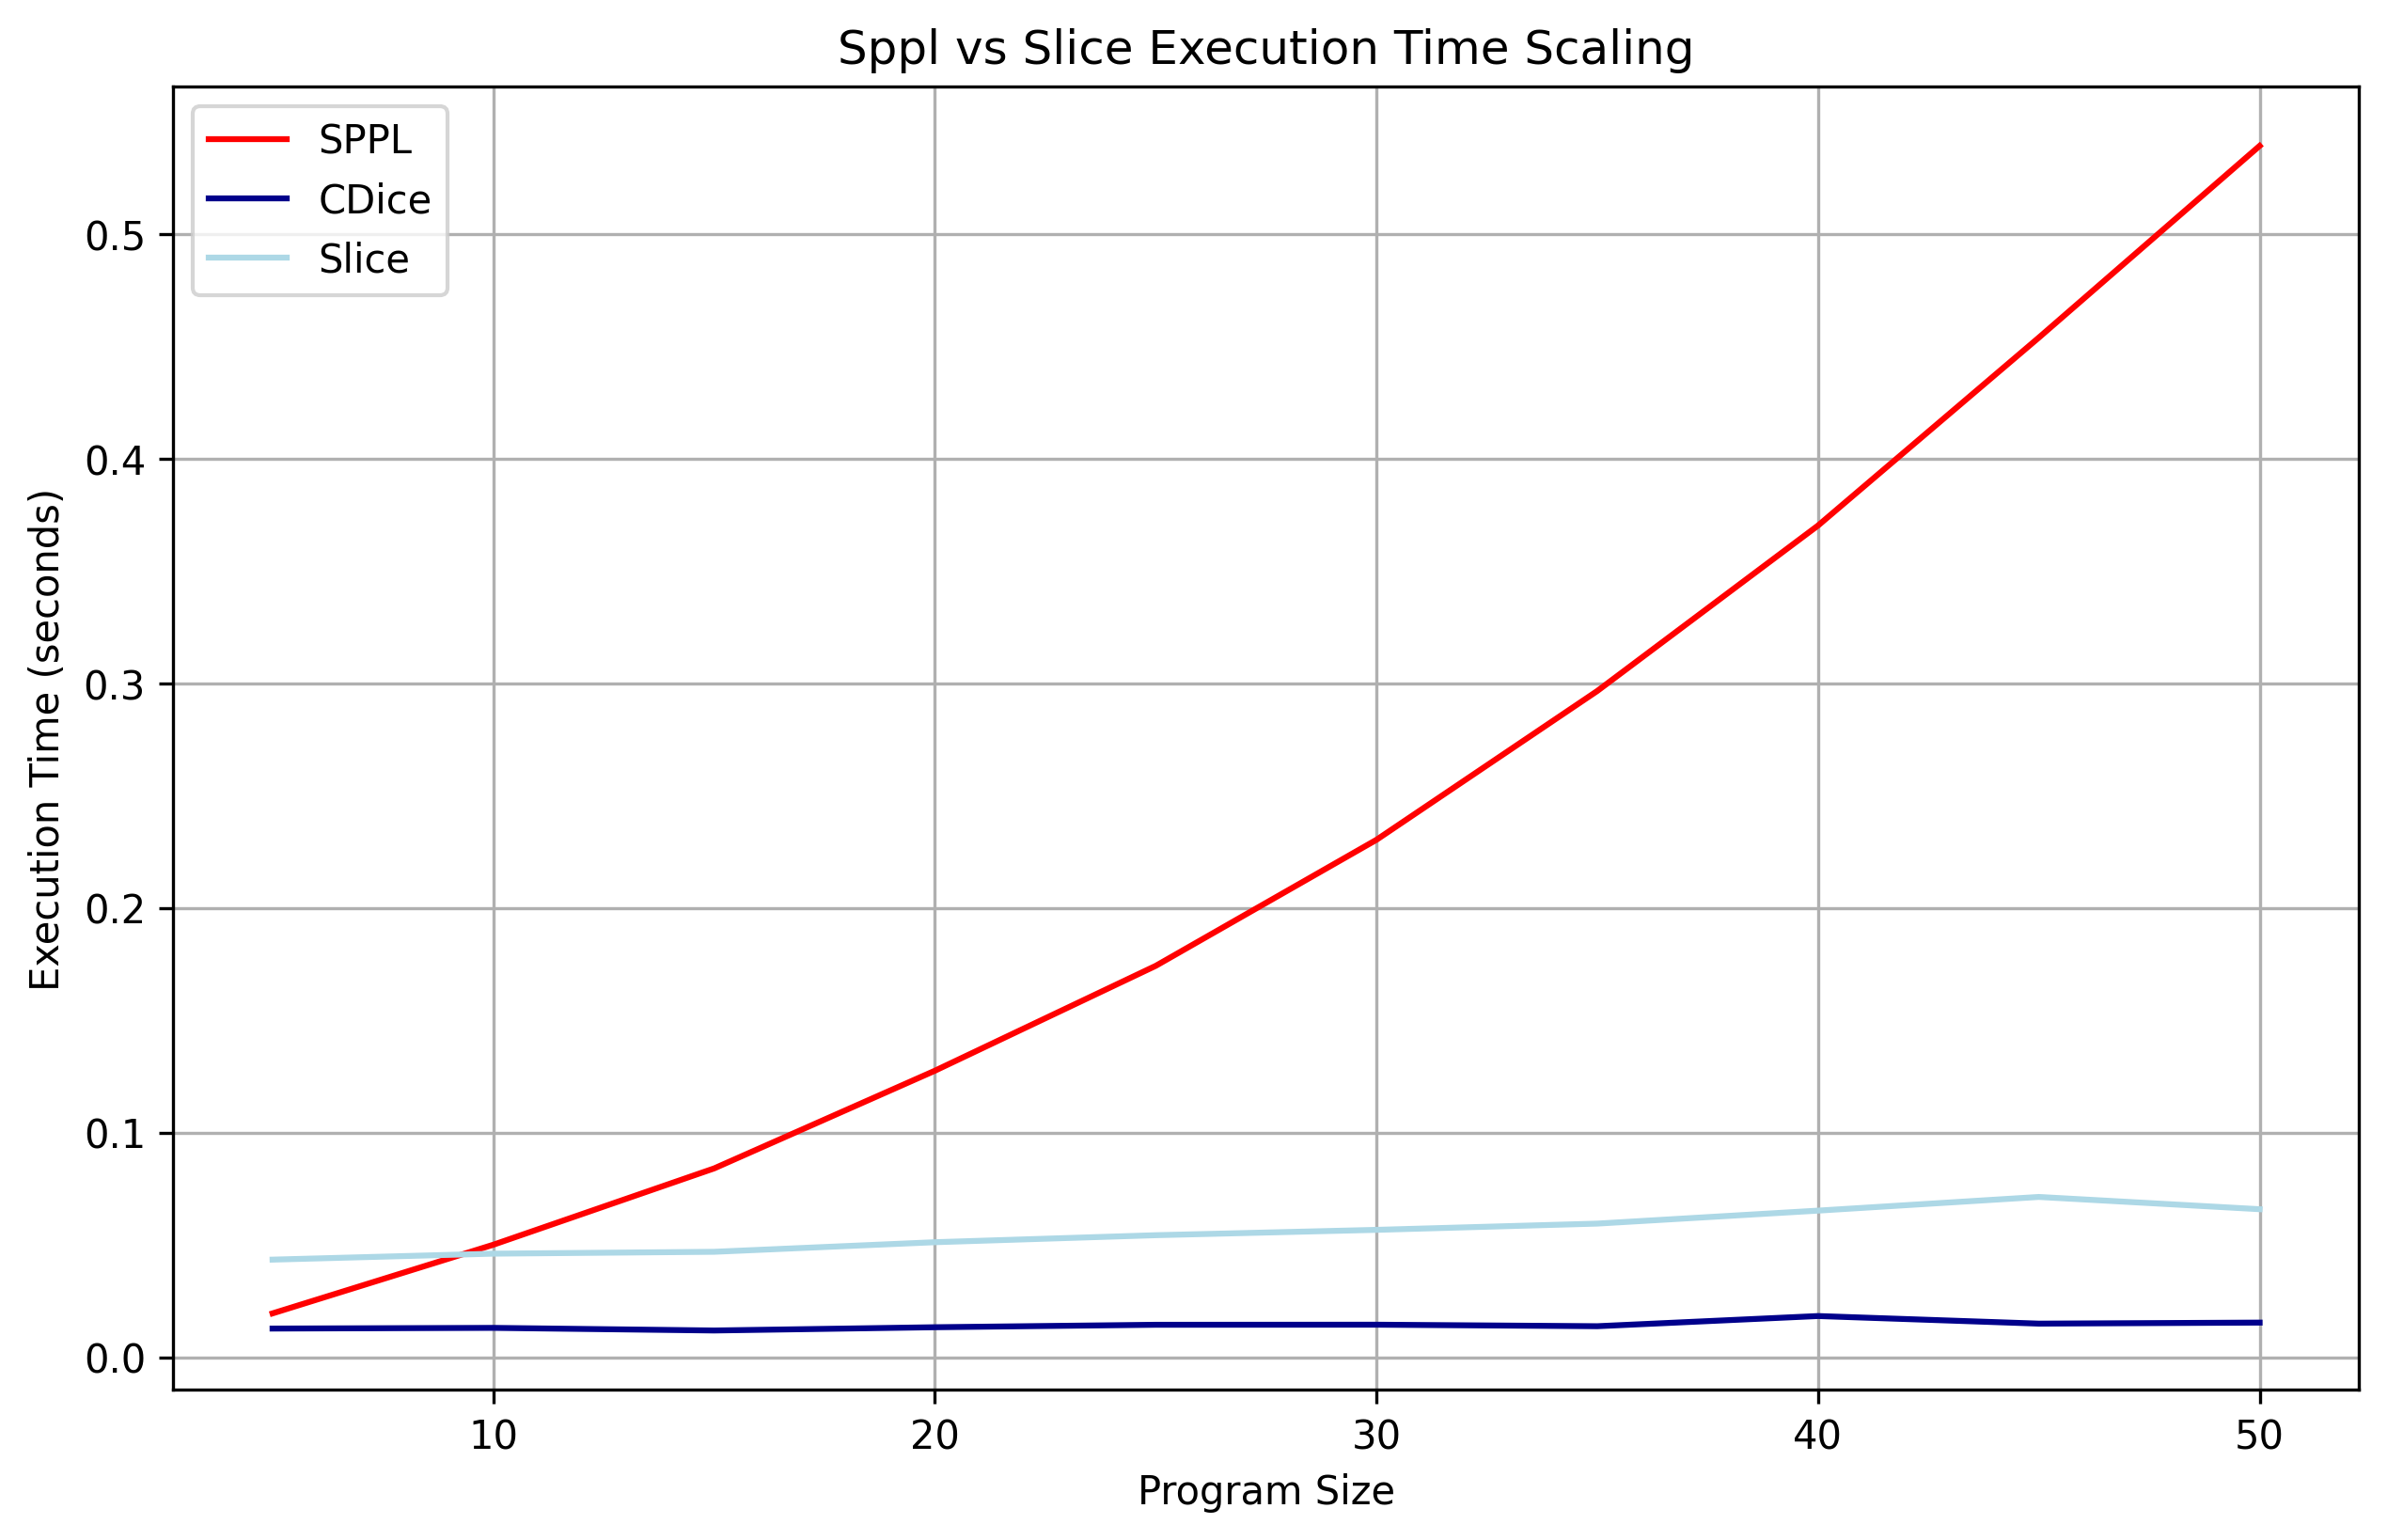
\includegraphics[width=\textwidth]{../images/scaling/build_alternating_guard_contdice_2.png}
\caption{Alternating Guard 2}
\label{fig:alt-benchmarks-b}
\end{subfigure}
\vspace{0.5em}
\begin{subfigure}{0.48\textwidth}
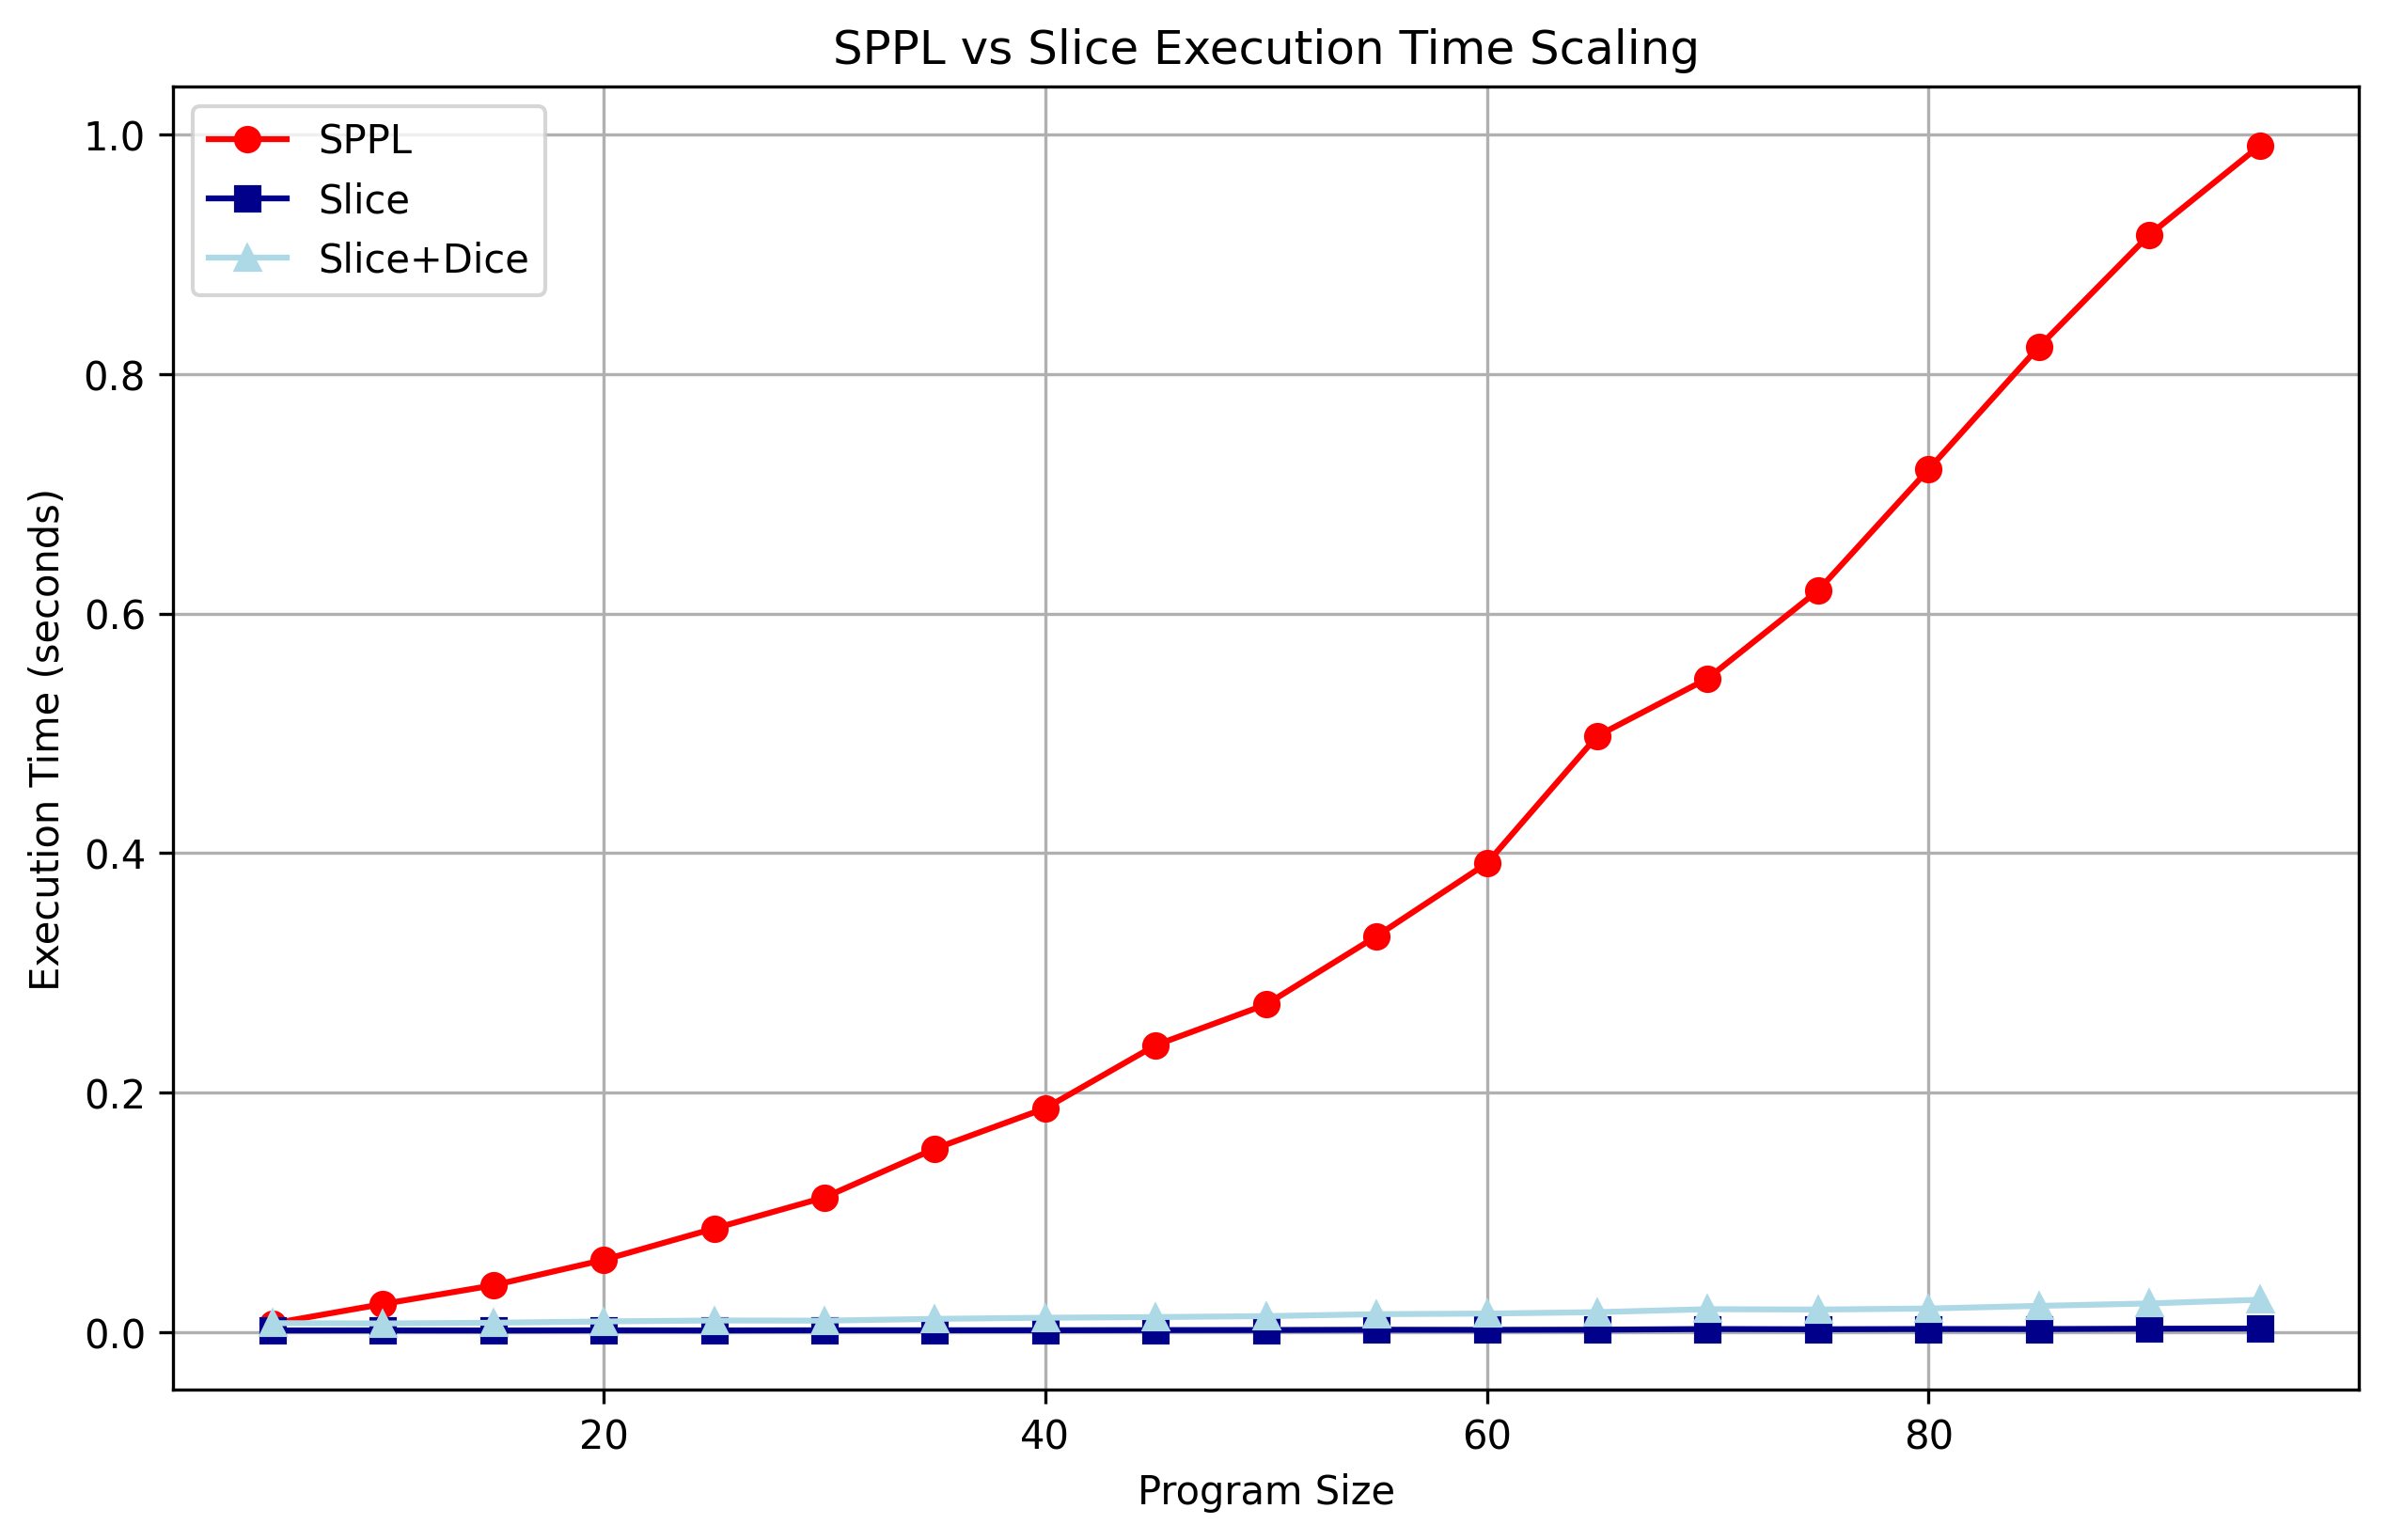
\includegraphics[width=\textwidth]{../images/scaling/build_alternating_guard_contdice_3.png}
\caption{Alternating Guard 3}
\label{fig:alt-benchmarks-c}
\end{subfigure}
\hfill
\begin{subfigure}{0.48\textwidth}
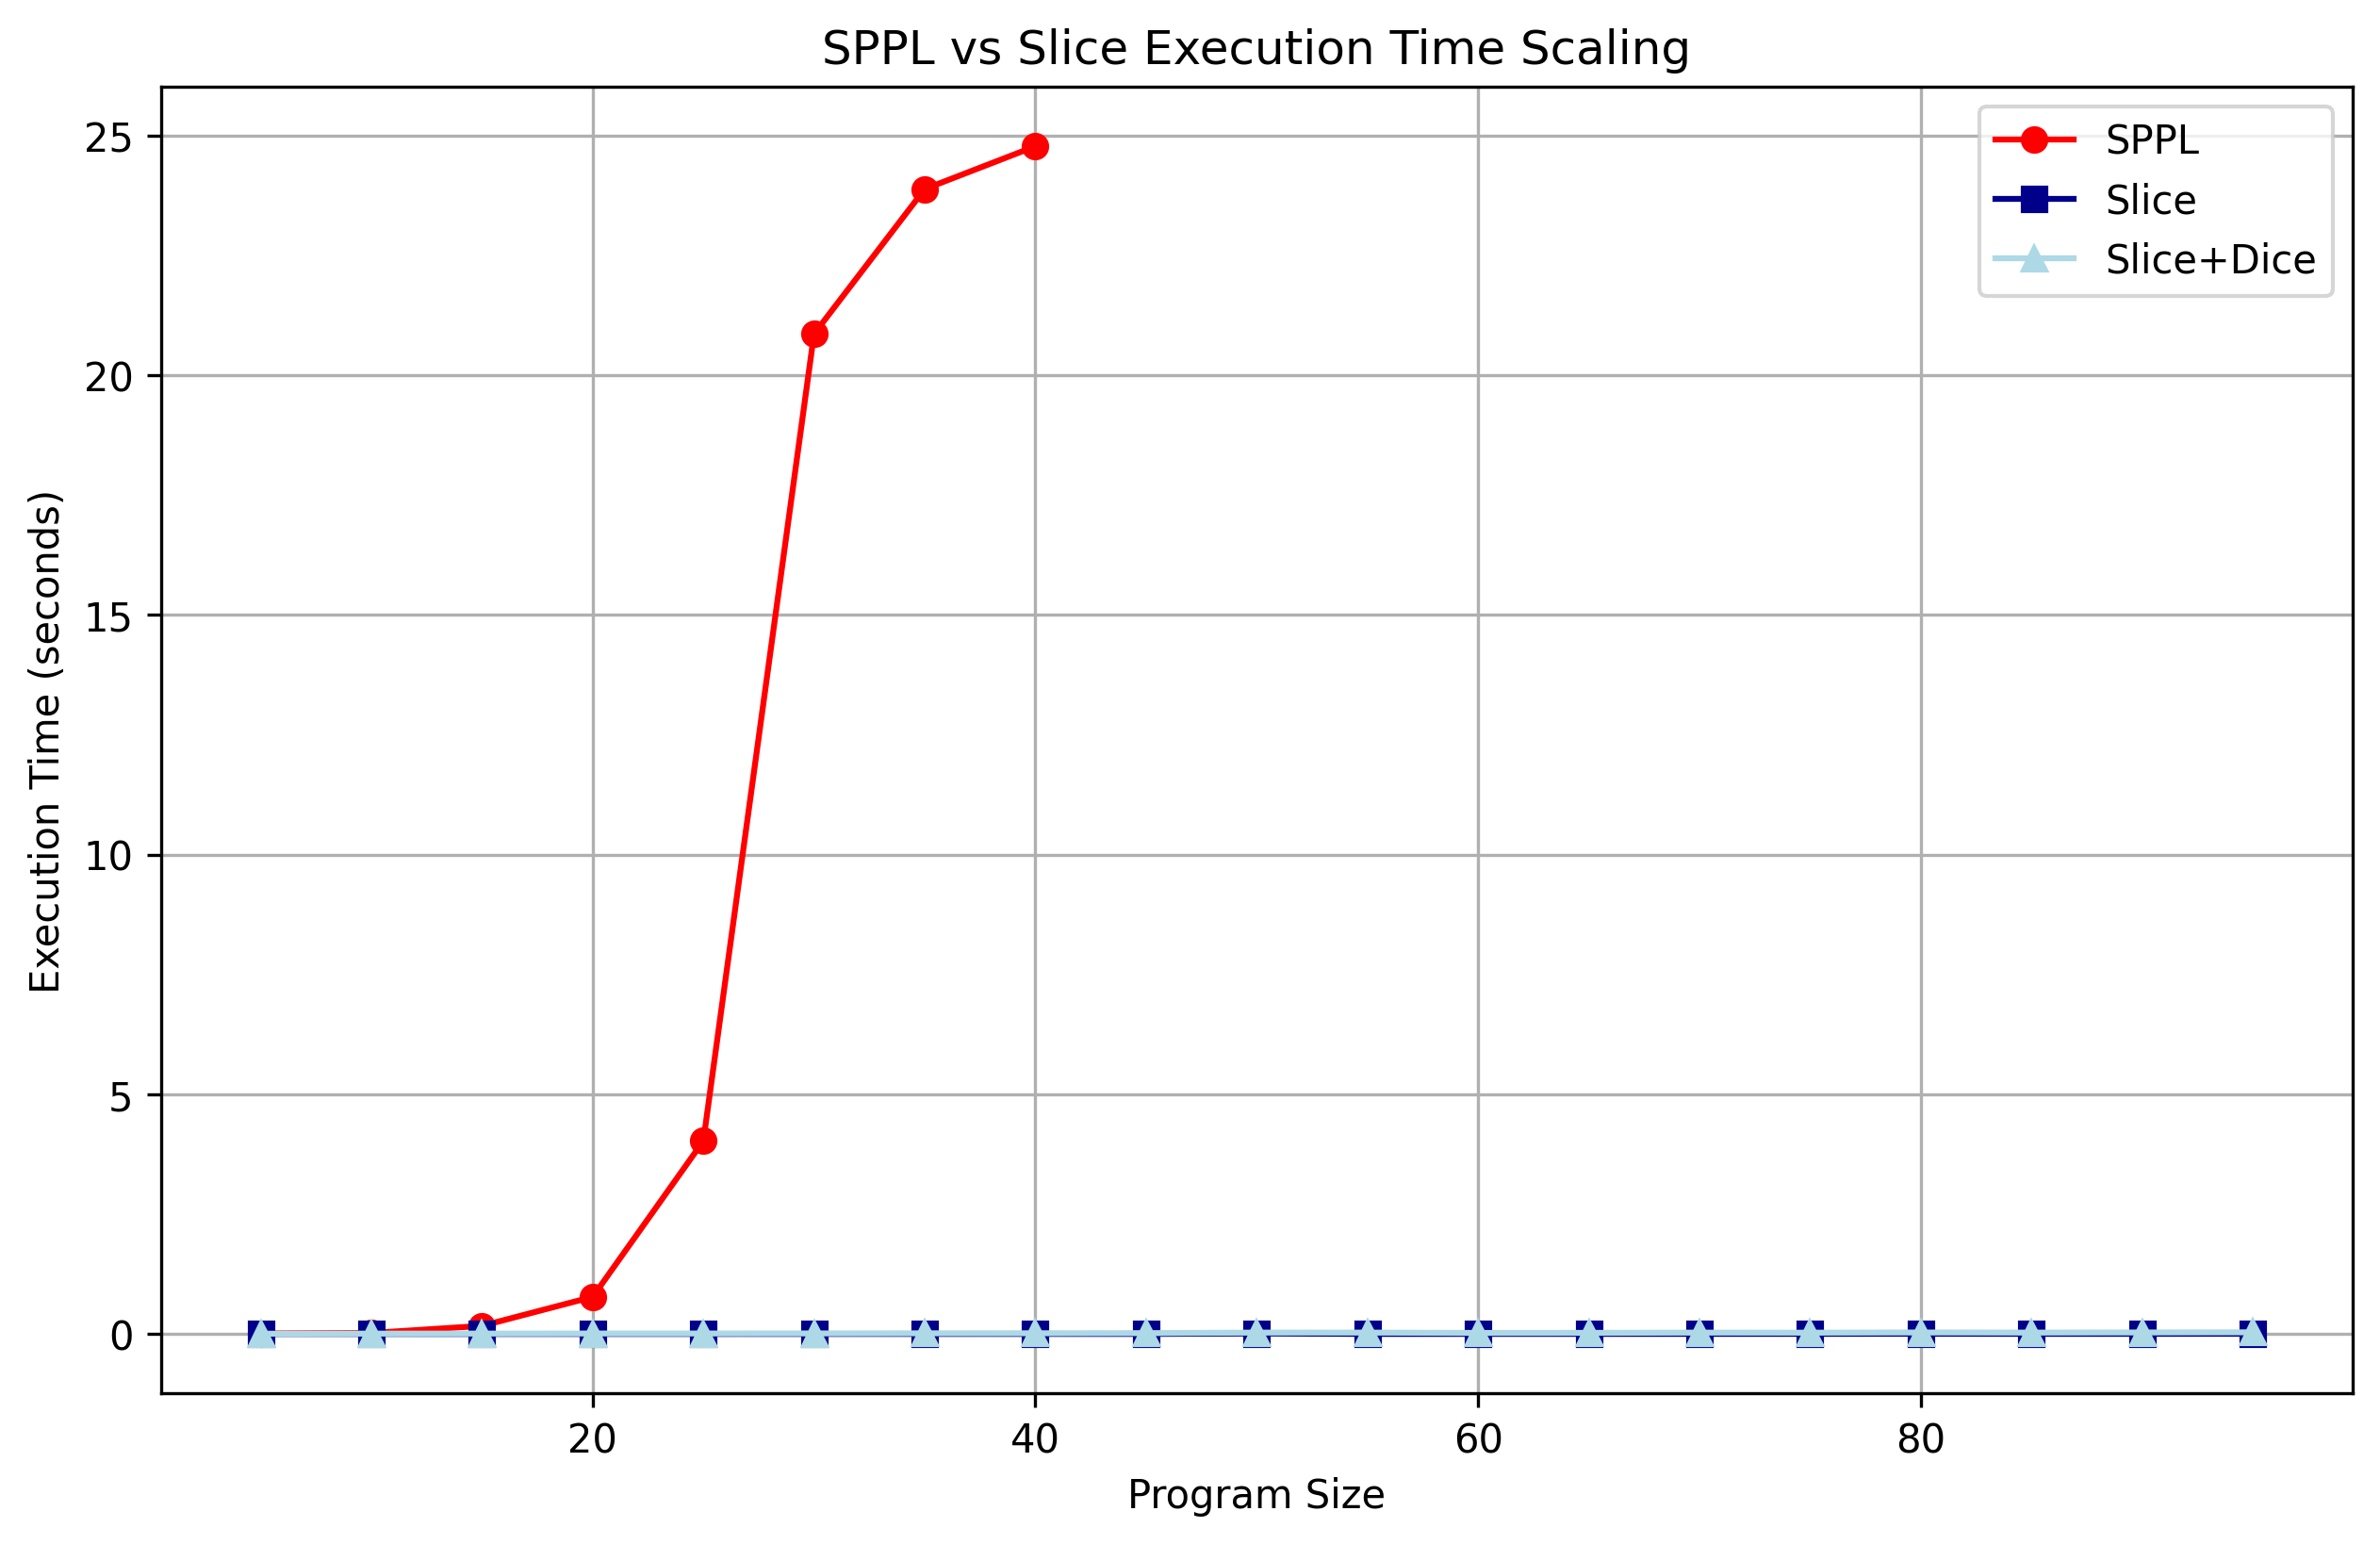
\includegraphics[width=\textwidth]{../images/scaling/build_random_alternating_guard_contdice.png}
\caption{Random Alternating Guard}
\label{fig:alt-benchmarks-d}
\end{subfigure}
\caption{Scaling results for alternating guard benchmarks. SPPL (red) times out early (between program sizes 20-30), while Slice continues to scale to large programs.}
\label{fig:alt-benchmarks}
\end{figure}

\paragraph{Results.} The scaling experiments demonstrate that Slice maintains near-linear scaling behavior while SPPL exhibits exponential growth and times out on larger programs. Across all seven benchmarks, Slice+Dice execution time remains under 0.5 seconds even for programs with 90+ variables and comparisons, while SPPL times out (at 300s) for programs as small as 20-30 variables. The Slice compilation phase alone (dark blue line) shows essentially constant time, indicating that the type-directed discretization algorithm scales extremely well.


\subsubsection{Decision Tree Benchmarks}
We evaluate Slice on decision tree models from the FairSquare suite with the following results:

\begin{table}[!t]
\centering
\begin{tabular}{lrrr}
\toprule
Benchmark & Slice+Dice (s) & SPPL (s) & Speedup \\
\midrule
DT4\_ind & 0.007 & 0.335 & 45.6× \\
DT4\_bn1 & 0.008 & 0.335 & 42.8× \\
DT4\_bn2 & 0.007 & 0.340 & 46.3× \\
DT14\_ind & 0.008 & 0.324 & 43.0× \\
DT14\_bn1 & 0.010 & 0.341 & 35.8× \\
DT14\_bn2 & 0.011 & 0.356 & 33.3× \\
DT16\_ind & 0.008 & 0.339 & 44.4× \\
DT16\_bn1 & 0.009 & 0.349 & 38.3× \\
DT16\_bn2 & 0.011 & 0.339 & 30.7× \\
DT44\_ind & 0.011 & 0.349 & 31.1× \\
DT44\_bn1 & 0.016 & 0.363 & 22.9× \\
DT44\_bn2 & 0.016 & 0.354 & 22.1× \\
\bottomrule
\end{tabular}
\caption{Execution times (seconds) for decision tree benchmarks}
\end{table}

\subsubsection{Clinical Trial Benchmark}
We evaluate Slice on a clinical trial model that uses discrete distributions to model treatment effectiveness:

\begin{table}[!t]
\centering
\begin{tabular}{lrrr}
\toprule
Benchmark & Slice+Dice (s) & SPPL (s) & Speedup \\
\midrule
Clinical Trial & 0.009 & 0.356 & 38.2× \\
\bottomrule
\end{tabular}
\caption{Execution times for clinical trial benchmark}
\end{table}


\subsection{Psi benchmarks}\label{sec:psi-benchmarks}
- describe benchmarks, cite paper
- simplications we made such as expanding out arrays
- graphs (slice + dice vs sppl vs bitblast)

\todo{Note: Psi benchmark files exist in dice/benchmarks/ but need to be ported to Slice syntax. Current .psi files include alarm, cancer, bayesian networks, etc.}

\subsection{Fairness benchmarks}\label{sec:fairness-benchmarks}
- describe benchmarks, cite paper
- simplications we made such as expanding out arrays
- graphs (slice + dice vs sppl vs bitblast)

\todo{Note: Fairness benchmarks need to be collected/created. The indian\_gpa example in examples/paper/ could be one fairness benchmark.}

\section{Related Work}
\label{sec:related}

\paragraph{Discrete-only probabilistic languages}  
Several recent systems achieve \emph{exact inference} by restricting models to finite, discrete random variables. \emph{Roulette} extends Racket with first-class support for finitely-supported distributions and leverages symbolic evaluation to compile queries into weighted model-counting problems, enabling scalable exact conditioning on complex programs~\cite{Moy2025Roulette}. \emph{Dice} follows a similar philosophy in an OCaml DSL, compiling discrete programs to weighted model counting to perform exact Bayesian updates even on thousands of Boolean and finite-categorical variables~\cite{Holtzen2020Dice}. Earlier work in probabilistic logic programming, most prominently \emph{ProbLog}, annotates Prolog facts with probabilities and reduces inference to weighted Boolean formulas that can likewise be solved exactly~\cite{DeRaedt2007ProbLog}. These languages demonstrate the power of exact reasoning, but by construction they \emph{cannot express continuous random quantities}; consequently they offer no built-in path for analysing models that naturally mix real-valued and discrete structure.  

\paragraph{Symbolic treatment of mixed models}  
\emph{SPPL} occupies an intermediate point on the design spectrum. By enforcing syntactic restrictions that guarantee every program can be translated into a finite \emph{sum-product expression}, SPPL supports models with both discrete and continuous components while still admitting \emph{symbolic} exact inference~\cite{Saad2021SPPL}. Rather than discretising the continuous parts, SPPL derives closed-form integrals when possible; exactness is retained for a narrow class of models. There is no mechanism for turning the remaining continuous structure into a discrete program that could reuse the powerful inference back-ends of Dice, Roulette, or ProbLog.

\paragraph{Continuous and hybrid PPLs with approximate inference}  
The majority of widely-used PPLs treat \emph{continuous} distributions as first-class and rely on approximate inference. Systems such as \emph{Stan} (C++), \emph{PyMC} (Python), \emph{Pyro} (Python on PyTorch), \emph{TensorFlow Probability} and its precursor \emph{Edward} expose rich continuous distributions and obtain posteriors with Hamiltonian Monte Carlo, variational inference, or sequential Monte Carlo~\cite{Carpenter2017Stan,Salvatier2016PyMC3,Bingham2019Pyro,Dillon2017TFP,Tran2016Edward}. These frameworks deliver high accuracy for differentiable densities but can struggle with discrete latent structure or discontinuities that arise after naïve discretisation. Crucially, none of them offers an automated pathway to convert continuous sub-expressions into discrete replacements that would make exact inference feasible.

\paragraph{Universal languages supporting both regimes}  
Universal or ``hybrid'' languages aim for expressiveness by embedding probabilistic primitives into general-purpose hosts. \emph{Anglican} (Clojure), \emph{WebPPL} (JavaScript), \emph{Figaro} (Scala) and \emph{Infer.NET} (C\#) permit arbitrary mixtures of discrete and continuous variables with inference based on importance sampling, Gibbs, expectation propagation, or lightweight MCMC~\cite{Tolpin2016Anglican,Goodman2014WebPPL,Pfeffer2009Figaro,Minka2018InferNET}. More recently, Julia-based systems such as \emph{Turing.jl} and \emph{Gen.jl} expose programmable inference interfaces, while \emph{Bean Machine} offers a declarative syntax atop PyTorch~\cite{Ge2018Turing,CusumanoTowner2019Gen,Tehrani2020BeanMachine}. Classic languages like \emph{Church} pioneered the ``evaluation-as-sampling'' view that underlies many of these systems~\cite{Goodman2008Church}. Discretization transformations are left entirely to the user and are not integrated with the inference engine.

\paragraph{Probabilistic program abstraction}
The work of \cite{Holtzen2018Abstraction} is perhaps most similar to our own in its aim to simplify probabilistic programs for easier inference.
They use ideas from abstract interpretation to transform a program with continuous and discrete random variables into a finite Boolean program based on user-provided predicates.
This *predicate abstraction* is proven to be \emph{distributionally sound}, meaning that for any query expressed in the predicate vocabulary, the abstract program gives the same probability as the concrete one.
Their method works by taking a set of predicates and automatically adding *completion* predicates to create a tight abstraction.
Inference then proceeds by querying the abstract Boolean program and using a concrete inference engine for sub-queries.
While this approach is powerful, it has several limitations.
The selection of predicates is left to the user, and a poor choice can lead to a coarse abstraction or a combinatorial explosion in the number of completion predicates.
Furthermore, the full automation of their technique is limited to loop-free programs.
Our work, in contrast, does not require user-provided predicates. Instead, \Slice{} automatically infers the necessary "cut points" from the program text using a novel type system, and our approach supports features like recursion.

\paragraph{Positioning of our work}  
Our contribution lies precisely at the intersection left open by the above lines of research. We propose a \emph{language-level transformation} that automatically discretises continuous sub-programs while preserving the semantics required for exact Bayesian reasoning in the discrete fragment. When discretization successfully translates all continuous distributions, we can translate the program into the finite domain accepted by Dice (or Roulette, or ProbLog), and inherit their fast exact inference without sacrificing the modelling convenience of continuous distributions. 
Empirically, our approach of discretizing programs and running them through Dice's inference engine achieves significantly faster runtimes compared to SPPL's symbolic methods, while maintaining exactness. Unlike continuous PPLs that settle for stochastic approximations, our approach bridges the gap between expressive modelling and fast exact computation. Partial discretization is also possible, and could be used to speed up inference without sacrificing expressiveness.

\medskip  
In summary, existing discrete PPLs excel at exactness but lack continuous support, symbolic languages like SPPL require restrictive structure and are slower than model counting approaches, and continuous or hybrid frameworks favour approximate inference. To our knowledge none of these systems automates the conversion of continuous programs into a discrete representation amenable to exact inference; our work addresses precisely that missing piece.

\paragraph{Future work}
In the future, we would like to extend our work to symbolically integrate tractable combinations of continous distributions beyond the cumulative distribution function.
We would also like to improve mixed continuous-discrete inference by partial discretization, summing out the discrete variables using weighted model counting techniques, and running the remaining continuous inference using standard continuous inference techniques.

\bibliographystyle{ACM-Reference-Format}
\bibliography{refs}



\end{document}